\documentclass[12pt,a4paper]{article}
\linespread{1,5}
\usepackage[utf8]{inputenc}
\usepackage[T2A]{fontenc}
\usepackage[russian]{babel}
\usepackage{amsmath}
\usepackage{amsfonts}
\usepackage{amssymb}
\usepackage{graphicx}
\usepackage{listings}
\usepackage[title,titletoc]{appendix}
\usepackage[left=30mm, top=20mm, right=15mm, bottom=20mm, nohead, footskip=10mm]{geometry}
\usepackage{indentfirst}
\author{Александр Лаптев}
\title{Создание информационной системы для организации работы предприятия}

\begin{document}

\begin{titlepage}
 \begin{center}
    \normalsize
    МИНИСТЕРСТВО НАУКИ И ВЫСШЕГО ОБРАЗОВАНИЯ \\
    РОССИЙСКОЙ ФЕДЕРАЦИИ \\
    ФГБОУ ВО «АЛТАЙСКИЙ ГОСУДАРСТВЕННЫЙ УНИВЕРСИТЕТ»
    \vfill
     
    Институт цифровых технологий, электроники и физики (ИЦТЭФ) \\
    Кафедра вычислительной техники и электроники (ВТиЭ)
    \vfill
     
    \textbf{Создание информационной системы для завода по производству и переработке цитрусовых.} \\
 \end{center}
\vfill
 
\newlength{\ML}
\settowidth{\ML}{«\underline{\hspace{3cm}}»}
\hfill\begin{minipage}{0.4\textwidth}
  Выполнил студент 595 гр.\\
  \underline{\hspace{\ML}} А.\,В.~Лаптев \\
  Проверил ст. преп. кафедры ВТиЭ\\
  \underline{\hspace{\ML}} И.\,А.~Шмаков \\
  «\underline{\hspace{1cm}}» \underline{\hspace{3cm}} 2021 г.
\end{minipage}%
\vfill
 
\begin{center}
  Барнаул, 2021 г.
\end{center}
\end{titlepage}

\tableofcontents
\newpage

\section*{Введение}
\addcontentsline{toc}{section}{Введение}
Цель: в заключительном задании по курсу требовалось создать информационную систему для предприятия, которое занимается производством цитрусовых и их последующей переработкой.
    
Требования к ИС:
\begin{enumerate}
    \item Наличие подсистем;
    
    \item Наличие всех видов справочников;
    
    \item Наличие документов (не менее 5 типов);
    
    \item Наличие регистров (не менее 5 типов);
    
    \item Наличие отчетов (не менее 10 видов).
\end{enumerate}

\section{Описание предприятия и логики его работы}
Задача созданной информационной системы заключалась в организации работы предприятия по производству и переработке цитрусовых. Предприятие самостоятельно выращивает различные виды цитрусовых и либо пускает их на переработку и продает физическим и юридическим лицам в виде какой-либо изготовленной продукции (например, в виде соков или лимонадов), либо сразу же продает выращенные фрукты свежими, без какой-либо переработки.

Таким образом, логика работы предприятия будет выглядеть следующим образом:

\begin{enumerate}
    \item Предприятие находится на полном самообеспечении и не использует услуги сторонних организаций для поставки фруктов или готовой продукции для ее дальнейшей переработки или реализации.

    \item В предприятии есть два подразделения: первое отвечает за выращивание цитрусовых и их продажу, второе --- за переработку части цитрусовых, для производства всевозможной продукции и продажу этой продукции.

    \item Для того, чтобы переработать цитрусовые в какую-то продукцию и затем продать ее, второму подразделению необходимо приобрести фрукты у первого. Факт приобретения <<сырья>> указывается в приходной накладной.

    \item Учет изготовленной продукции, которая была направлена на реализацию, ведется в товарной накладной. Реализация изготовленной продукции ведется вторым подразделением.

    \item Среди прочего, предприятие оказывает услуги по возврату продукции (будь то фрукты или изготовленная из них продукция), которая не удовлетворила клиента качеством.

    \item Помимо этого, предприятие самостоятельно отслеживает свежесть продукции на своих складах и проводит утилизацию продуктов, для которых истек срок хранения (были возвращены). Эти изменения отображаются в соответствующей накладной.
\end{enumerate}

Также, на предприятии реализована централизованная схема доставки товаров на склады, если в этом есть необходимость. А именно, все фрукты и готовая продукция сначала попадают на основной склад, а уже после этого, по желанию руководства, товары могут расходоваться либо с основного склада (если клиентов немного), либо перераспределяться для розничной и оптовой торговли в соответствующие склады(если у предприятия большое количество клиентов или много продукции для реализации).

\section{Описание информационной системы}
Согласно заданию преподавателя, информационная система разрабатывалась для завода по производству и переработке цитрусовых.

Информационная система разрабатывалась с использованием 1С версии 8.3 (учебная версия).

Изначально, были реализованы все необходимые требования к информационной системе.

Первым, что нужно было сделать это разбить будущую систему на более мелкие составные части (подсистемы). В моем случае подсистемы получились следующими:

\begin{enumerate}
    \item Бухгалтерия
    
    \item Учет Сырья
    
    \item Учет Готовой Продукции
    
    \item Расчет Зарплаты
    
    \item Продажи
    
    \item Предприятие
\end{enumerate}

Затем были созданы справочник четырех типов. Среди справочников были созданы следующие:

\begin{enumerate}
    \item Клиенты --- при создании был выбран тип: простой справочник. Справочник включает в себя список клиентов предприятия (физические и юридические лица) в количестве 15 человек.
    
    \begin{figure}[!ht]
        \centering
        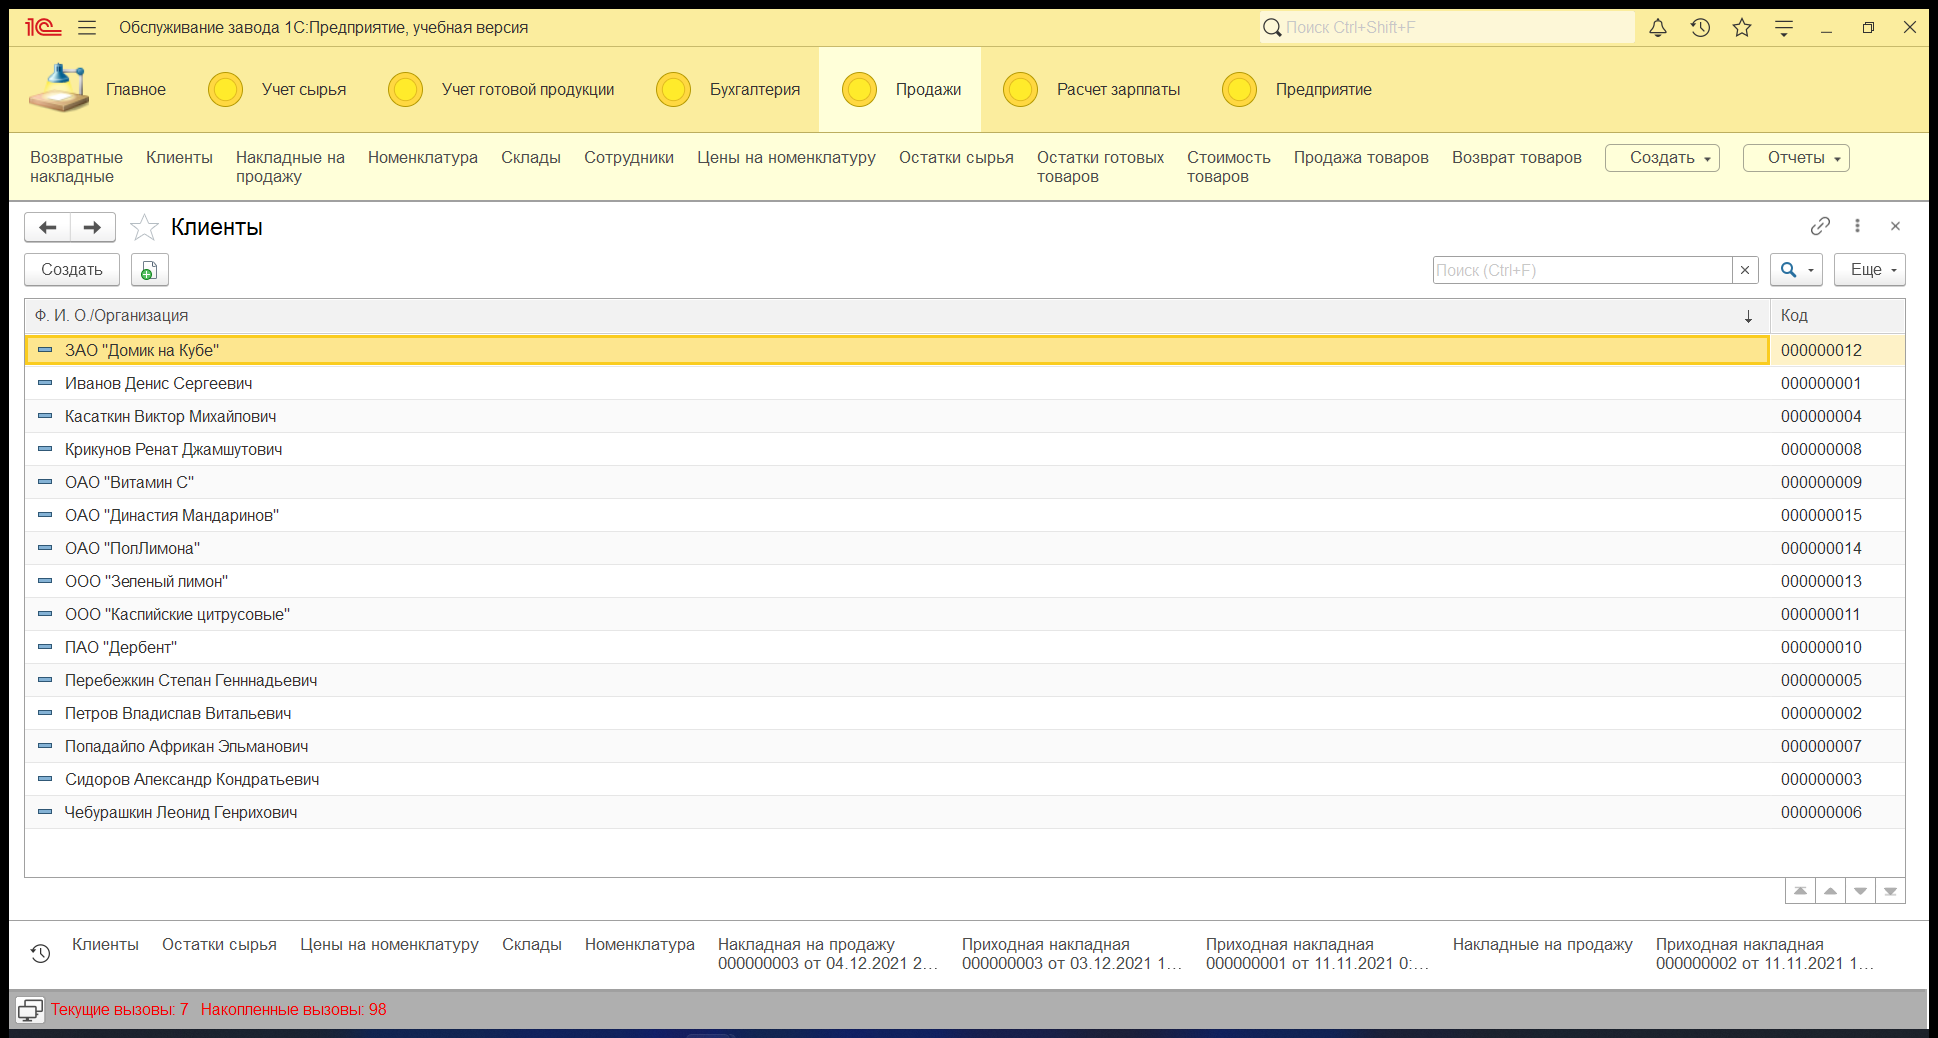
\includegraphics[scale=0.4]{Простой справочник.png}
        \caption{Простой справочник --- Клиенты}
        \label{fig:client}
    \end{figure}
    
    \item Сотрудники --- при создании был выбран тип: справочник с табличной частью. Справочник включает в себя список сотрудников предприятия (15 человек) с указанием их должности, предыдущего места работы и времени работы в предыдущей организации.
    
    \begin{figure}[!ht]
        \centering
        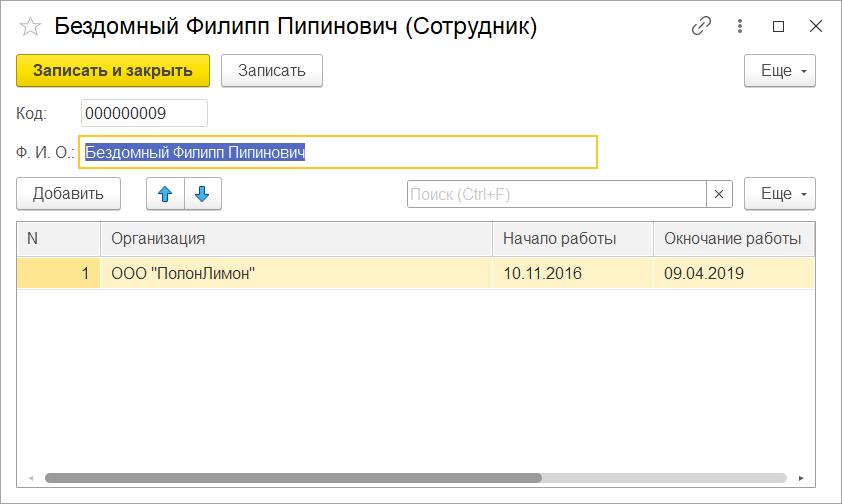
\includegraphics[scale=0.9]{Справочник с табличной частью.png}
        \caption{Справочник с табличной частью --- Сотрудники}
        \label{fig:worker}
    \end{figure}
    
    \item Склады --- при создании был выбран тип: справочник с предопределенными элементами. В качестве предопределенного элемента выступает основной склад, помимо которого присутствуют, также, оптовый и розничный.
    
    \begin{figure}[!ht]
        \centering
        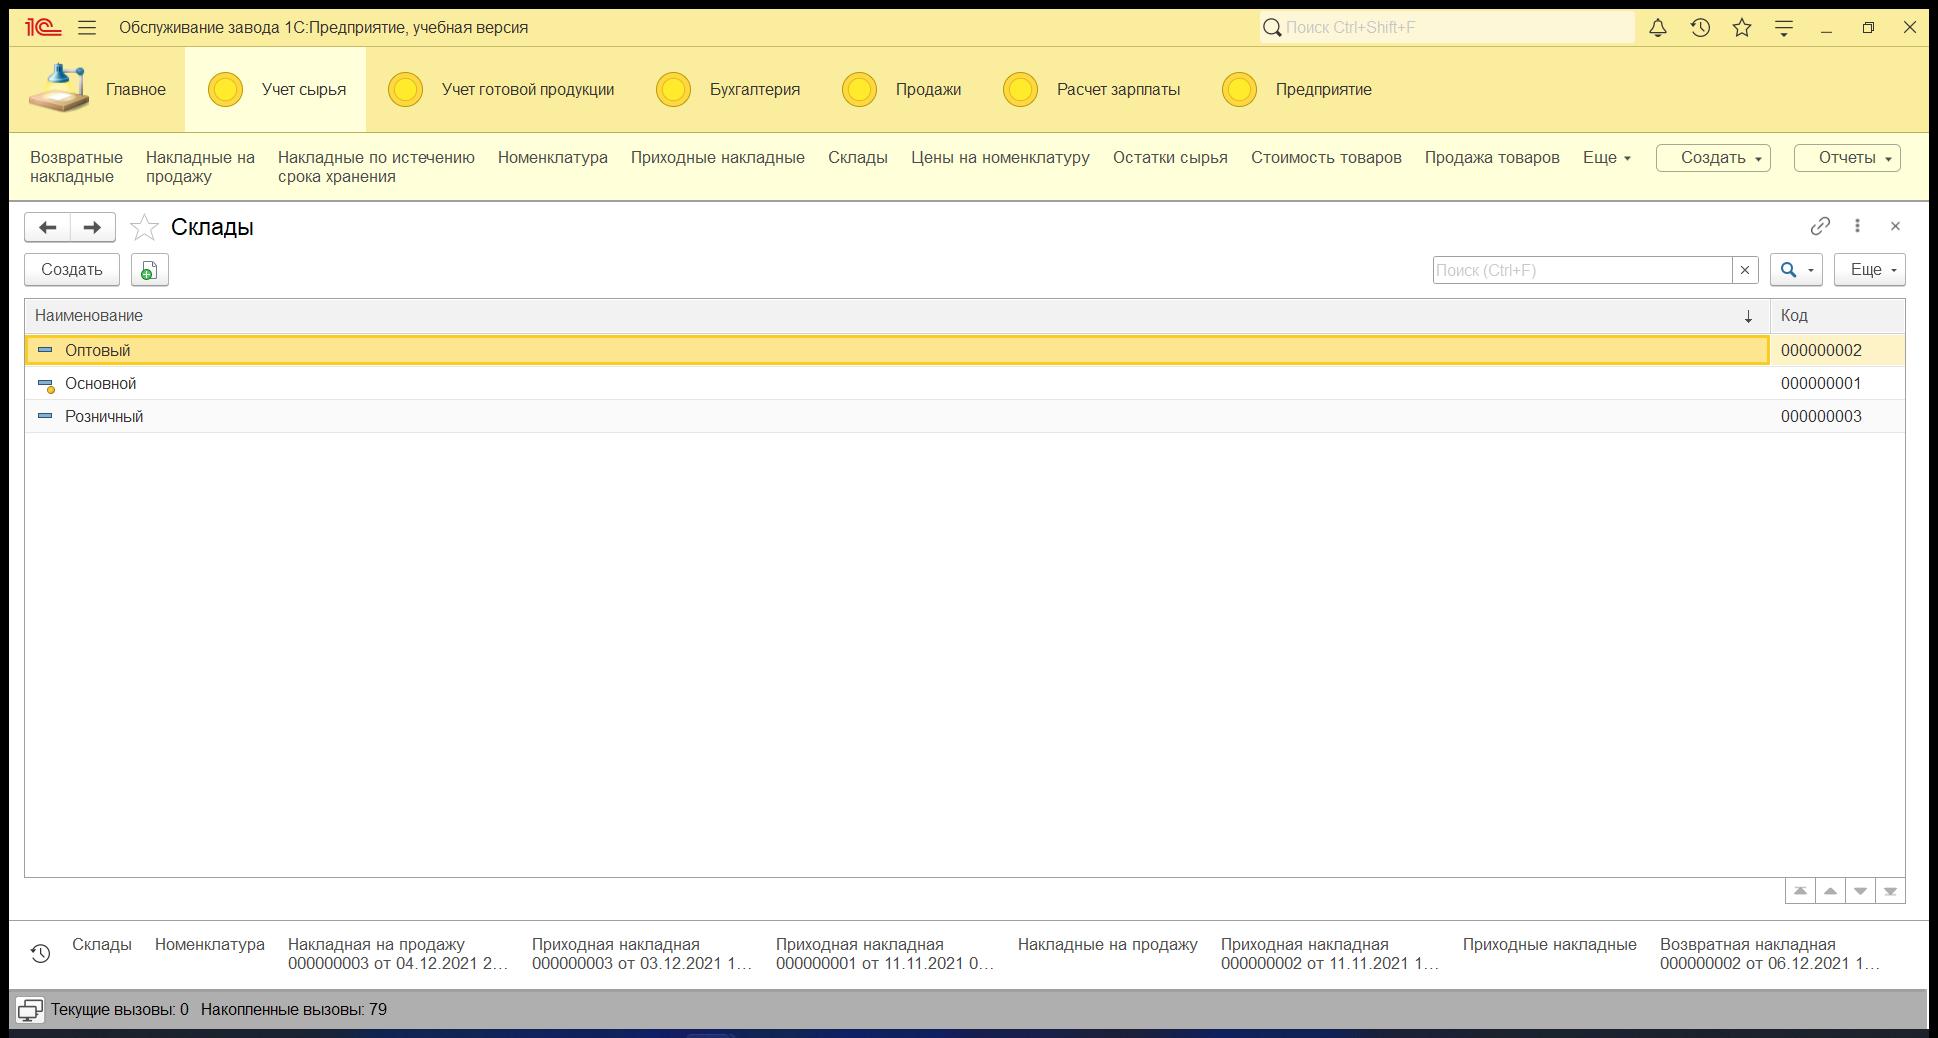
\includegraphics[scale=0.4]{Справочник с предопределенными элементами.png}
        \caption{Справочник с предопределенными элементами --- Склады}
        \label{fig:warehouse}
    \end{figure}
    
    \item Номенклатура --- при создании был выбран тип: иерархический справочник. Данный справочник включает в себя все наименования товаров, которые может производить и продавать предприятие. Все товары принадлежат к определенным категориям, которые и создают определенную иерархию в справочнике.
    
    \begin{figure}[!ht]
        \centering
        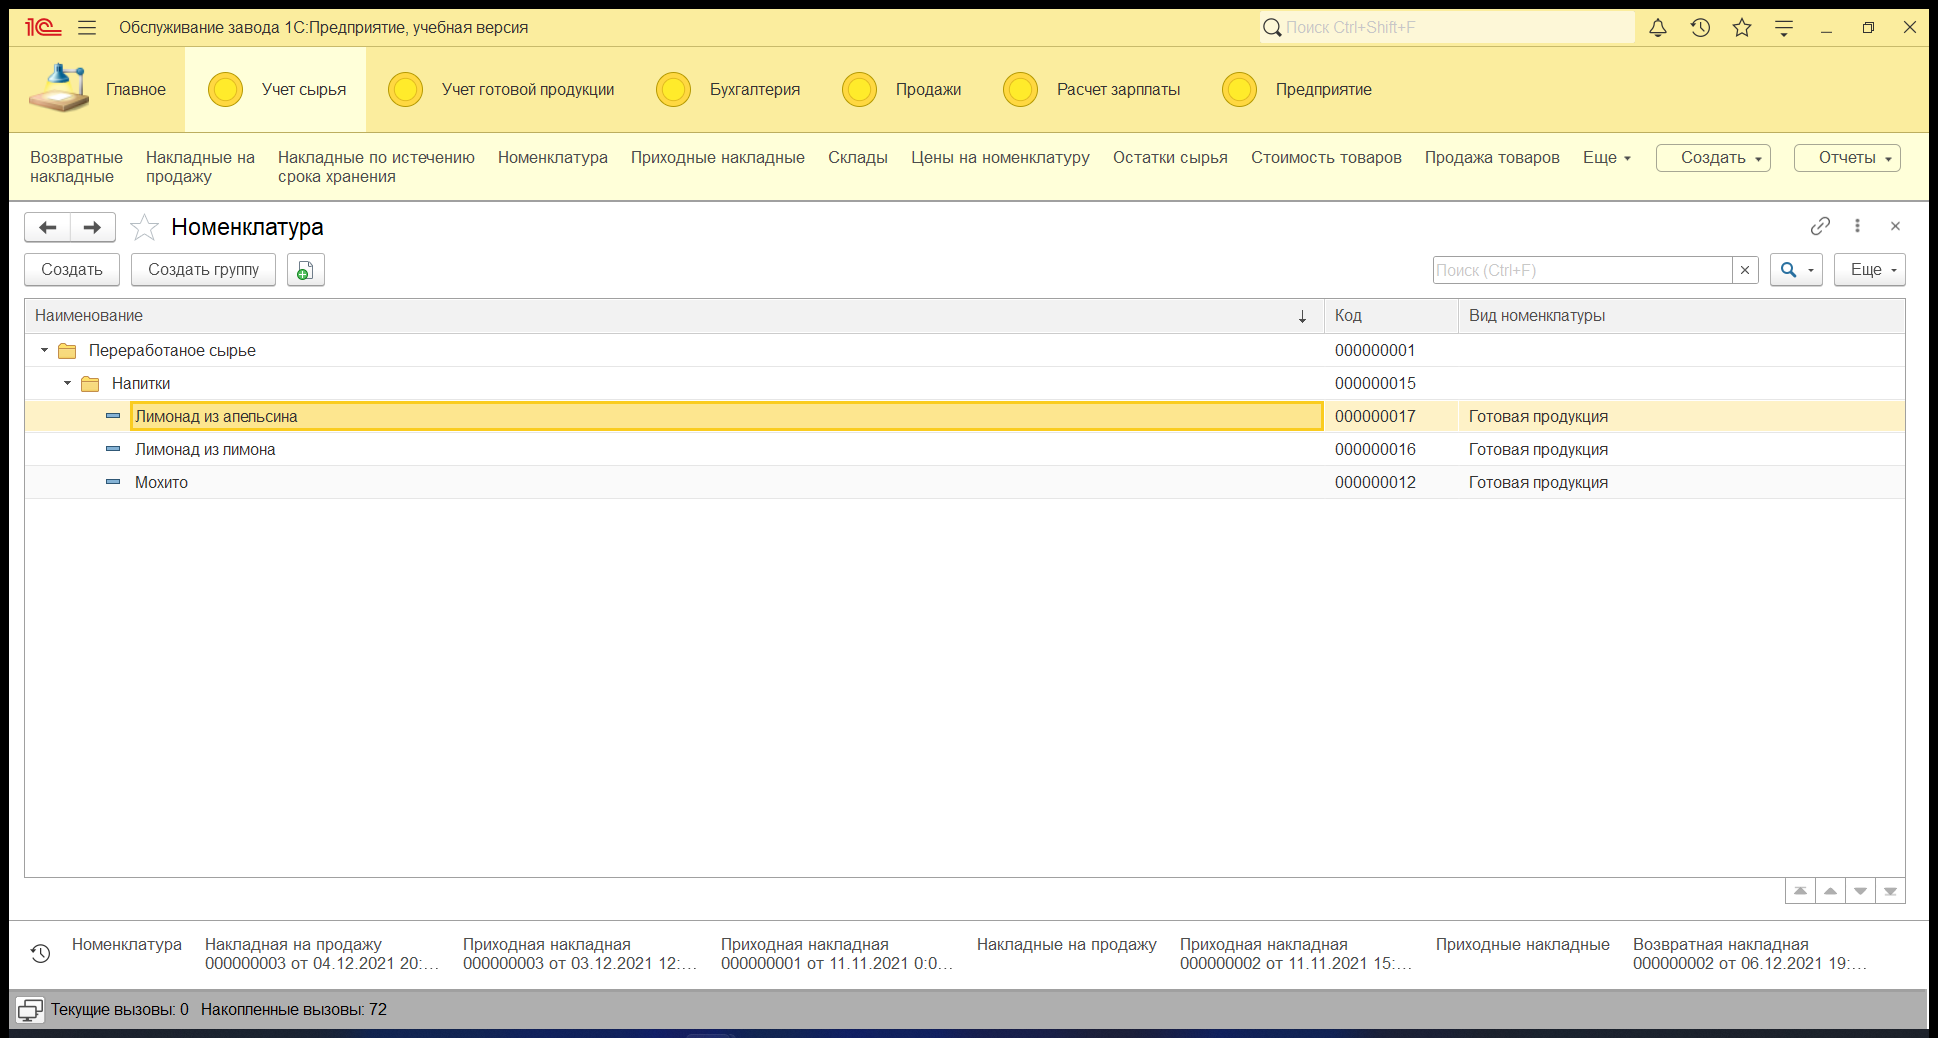
\includegraphics[scale=0.4]{Иерархический справочник.png}
        \caption{Иерархический справочник --- Номенклатура}
        \label{fig:Nomenclature}
    \end{figure}
    \newpage
\end{enumerate}

Следующим шагом, было создание документов, которые будут отражать в себе движения фруктов и изготовленной продукции между подразделениями предприятия и между предприятием и клиентами.

Для выполнения минимальных требований к информационной системе (5 документов) были введены следующие документы:

\begin{enumerate}
    \item Приходная накладная --- документ служит для того, чтобы учитывать фрукты, которые могут быть отправлены на переработку другому подразделению либо проданы клиентам в <<сыром>> виде.
    
    \item Товарная накладная --- этот документ служит для того, чтобы учитывать изготовленную продукцию, которая может быть реализована среди клиентов.
    
    \item Накладная на продажу --- в документе отражаются товарно-денежные отношения между предприятием и клиентами (покупка клиентом определенного вида продукта в определенных количествах по определенной стоимости).
    
    \begin{figure}[!ht]
        \centering
        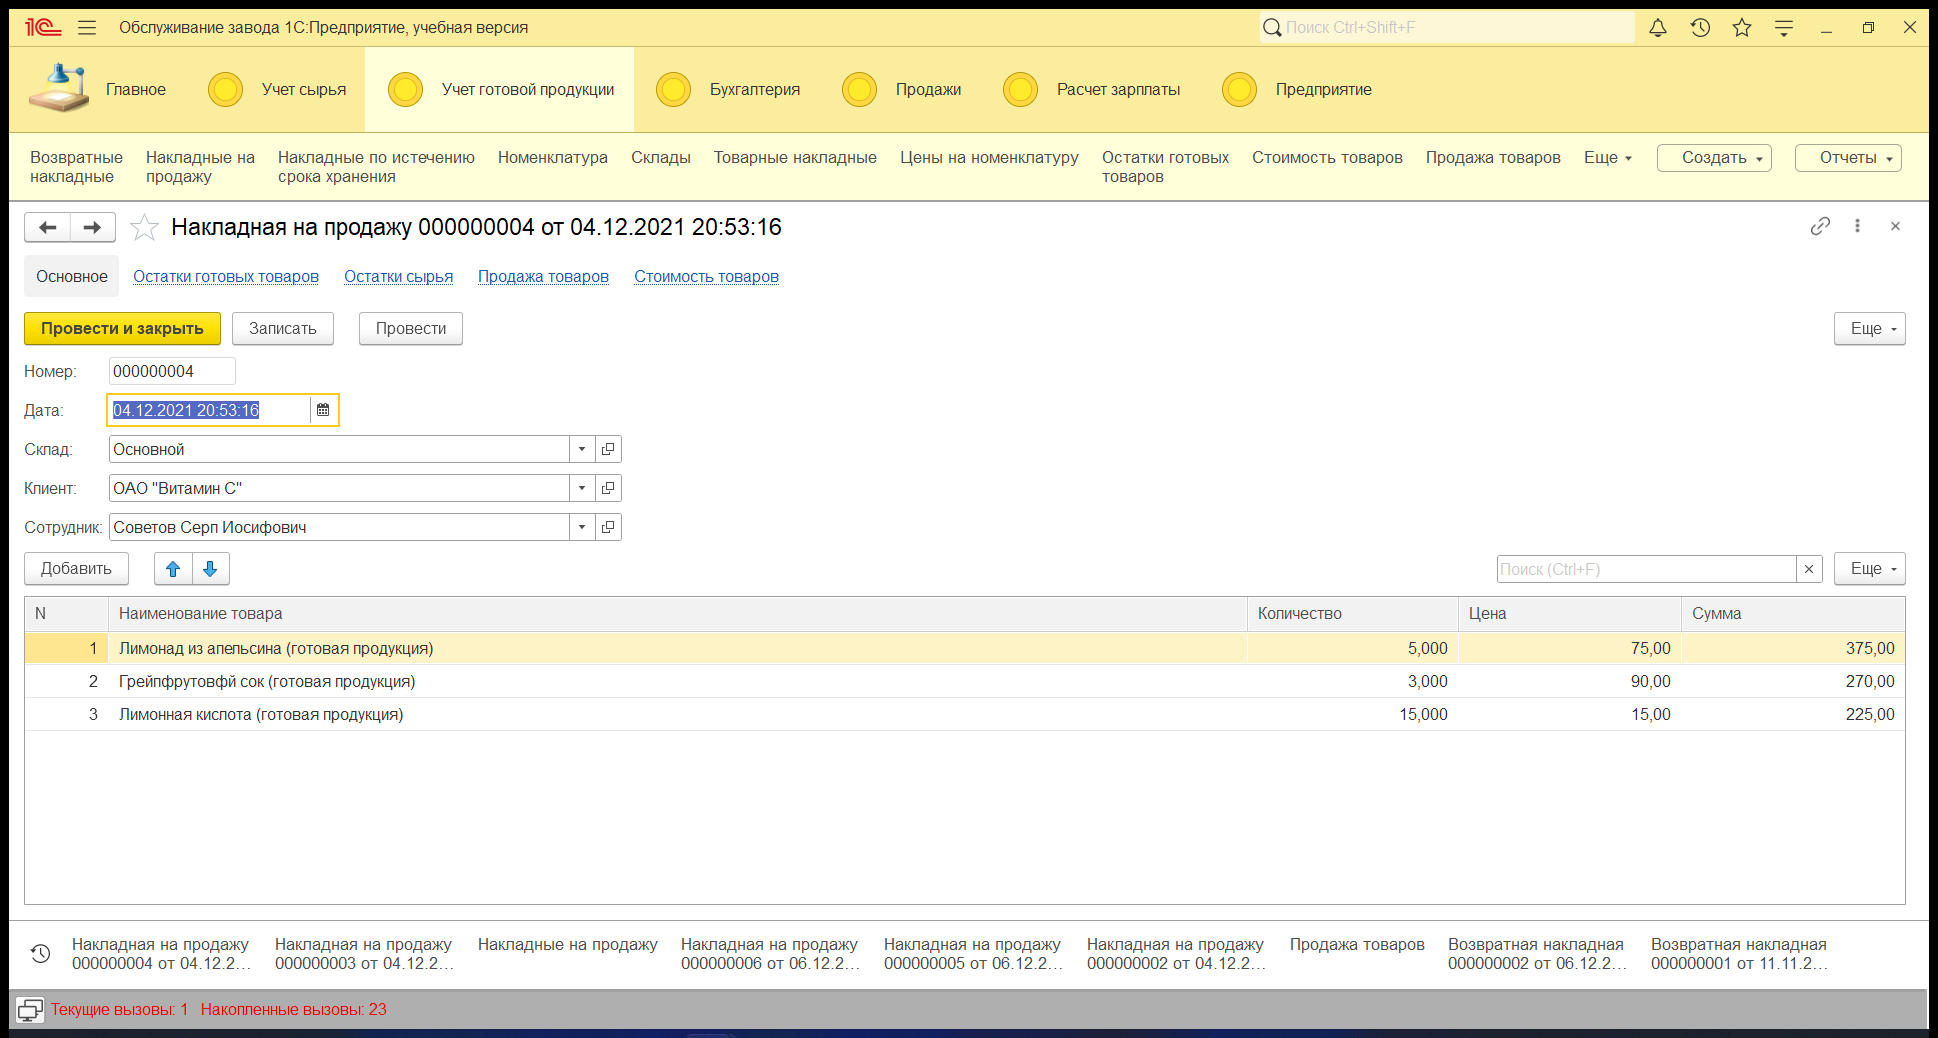
\includegraphics[scale=0.4]{Пример документа.png}
        \caption{Вид документа на примере Накладной на продажу}
        \label{fig:document}
    \end{figure}
    
    \item Возвратная накладная --- документ нужен для того, чтобы отражать возврат каких-либо товаров клиентом, в связи с их неудовлетворительным качеством или по иным причинам. При этом, для упрощения экономической модели будем исходить из того, что возвращенные товары тут же утилизируются.
    
    \item Накладная по истечению срока хранения --- документ присутствует для отражения утилизации некачественных товаров, которые были возвращены недовольными клиентами. Для упрощения экономической модели будем считать, что все товары, которые производит предприятие реализуются до момента истечения их срока годности.
\end{enumerate}

После создания всех необходимых документов был осуществлен переход к созданию регистров. Согласно минимальным требованиям необходимо создать 5 типов регистров.

Для данной информационной системы были созданы следующие регистры:

\begin{enumerate}
    \item Регистры накопления:
    
        \begin{enumerate}
            \item Остатки сырья --- этот регистр нужен для того, чтобы накапливать информацию о приходе на склад и расходе со склада фруктов в <<сыром>> виде.
            
            \begin{figure}[!ht]
                \centering
                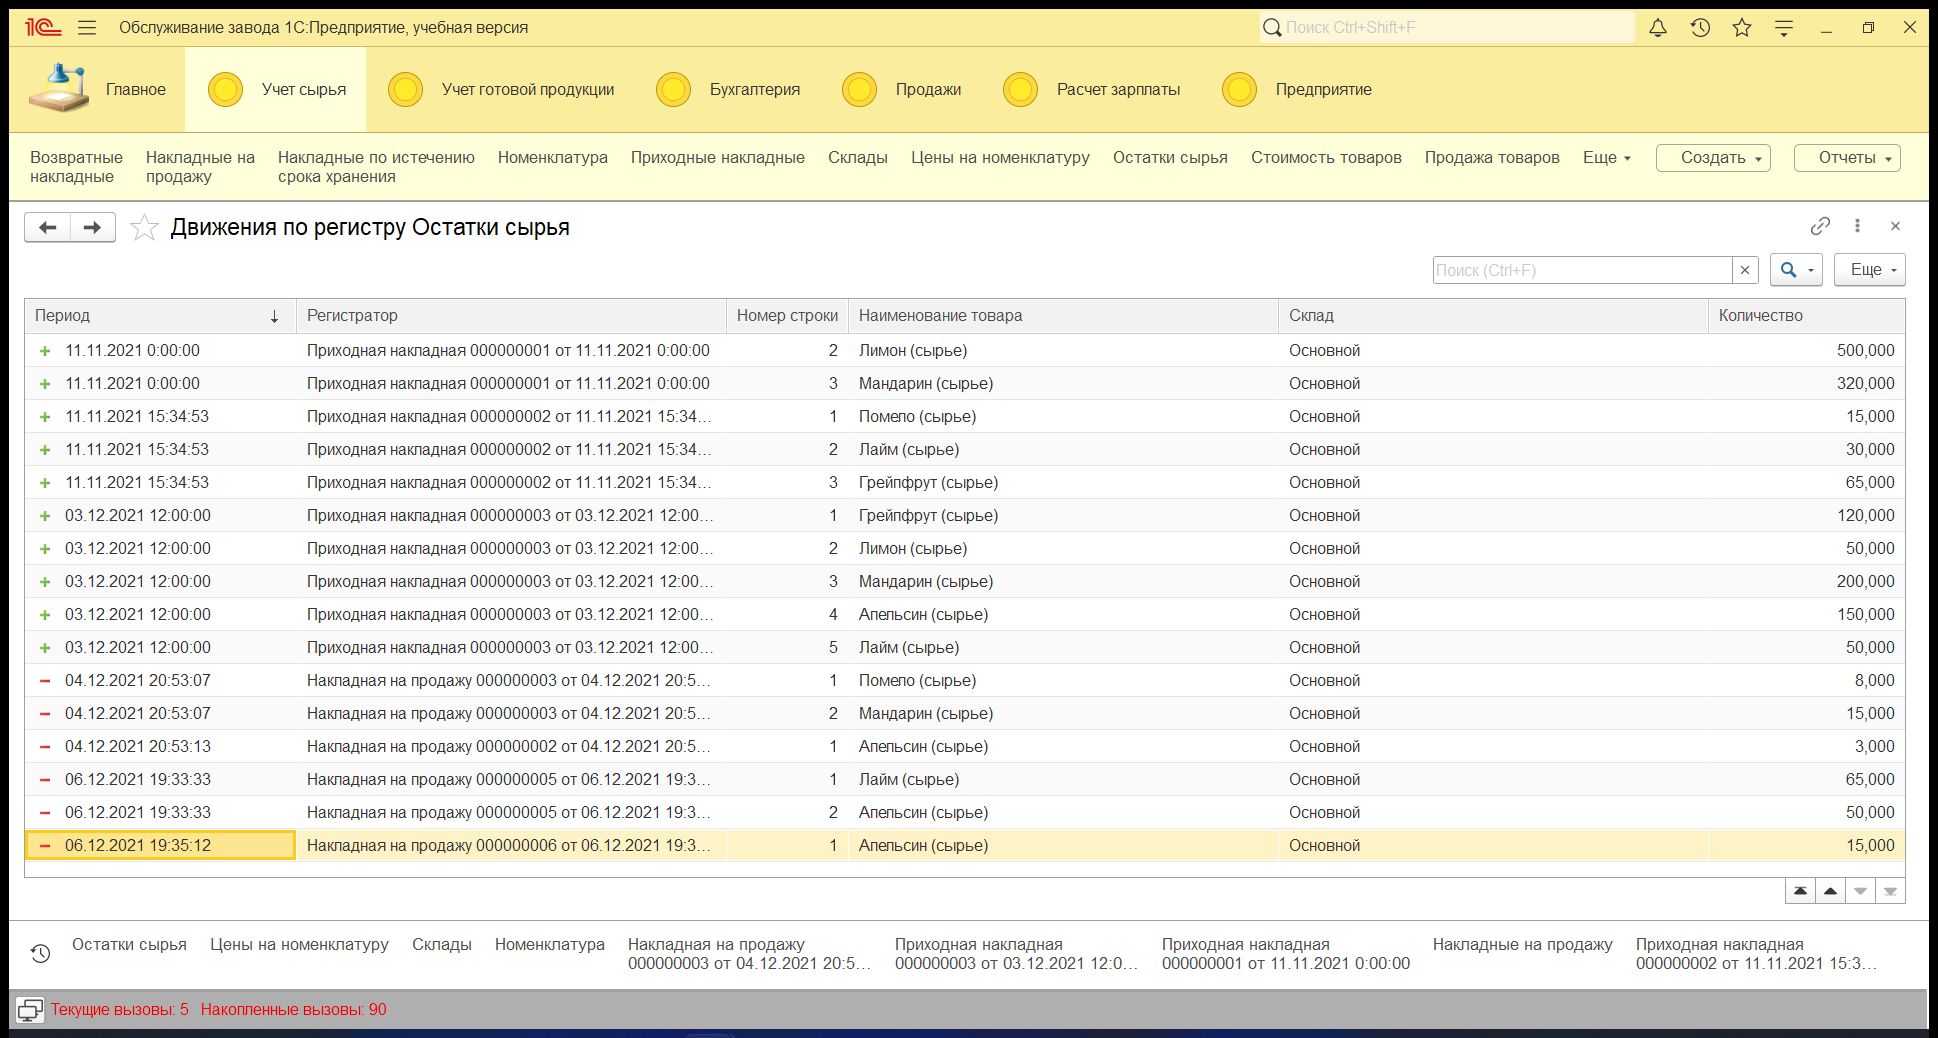
\includegraphics[scale=0.4]{Пример регистра накоплений.png}
                \caption{Вид регистра накоплений Остатки сырья}
                \label{fig:accumulation}
            \end{figure}
            
            \item Остатки готовых продуктов --- этот регистр служит для того, чтобы накапливать информацию о приходе на склад и расходе продукции, полученной в результате переработки цитрусовых.
            
            \item Продажа товаров --- регистр предназначен для накапливания информации о товарах, которые были реализованы как в <<сыром>>, так и в переработанном виде.
            
            \item Возврат товаров --- в данном регистре накапливается информация о тех товарах, которые были возвращены клиентами в связи с неудовлетворительным качеством.
            
            \item Списание товаров --- регистр служит для накопления информации о товарах, которые списываются со склада в связи с истечением срока хранения (для данной экономической модели --- товары, которые были возвращены клиентами).
            
            \item Стоимость товаров --- регистр накапливает информацию о стоимости товаров, которые указаны в товарной накладной. Стоимость для товара проставляется <<по среднему>> и не требует непосредственного ввода пользователем.
        \end{enumerate}
        
    \item Регистры сведений:
    
        \begin{enumerate}
            \item Цены --- данный регистр сведений отвечает за изменение цен на номенклатуру со временем, в определенных временных пределах. С его помощью предприятие может изменять цены на свою продукцию в любой момент времени.
            
            \begin{figure}[!ht]
                \centering
                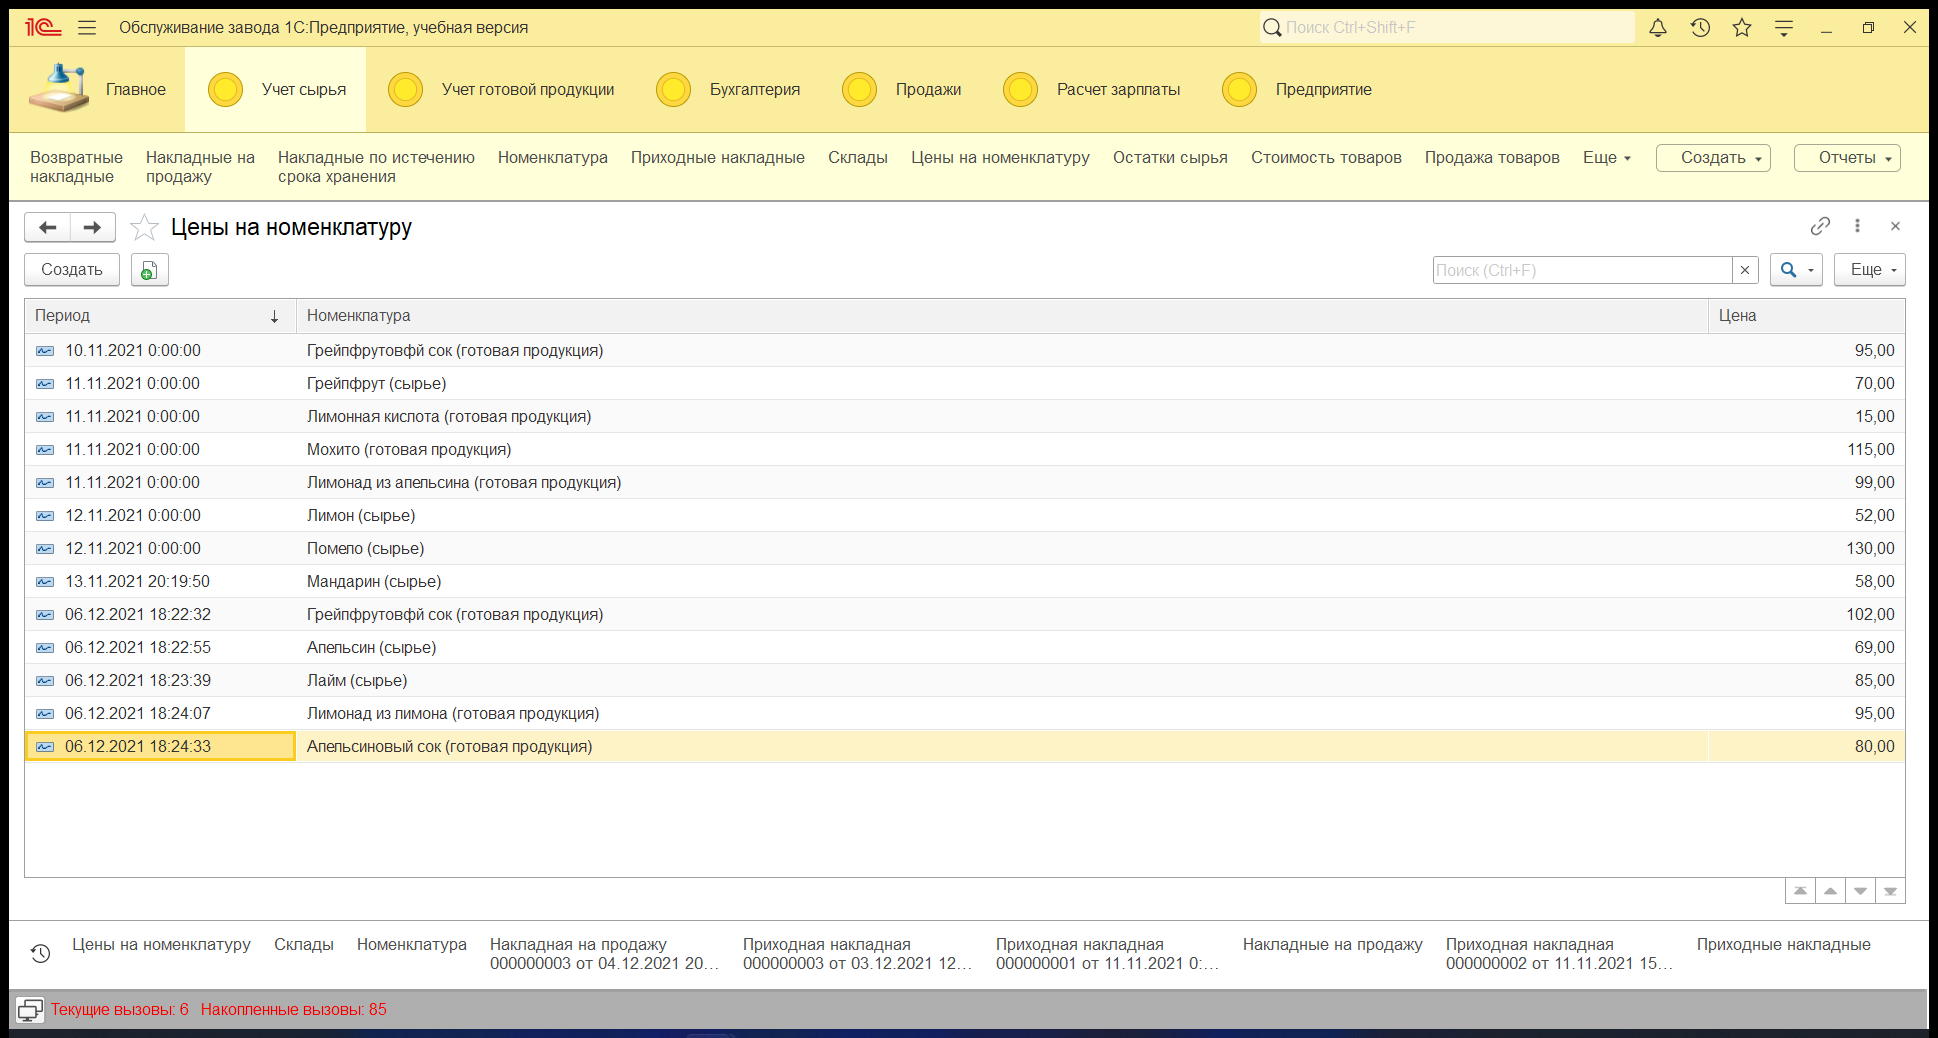
\includegraphics[scale=0.4]{Пример регистра сведений.png}
                \caption{Вид регистра сведений Цены}
                \label{fig:information}
            \end{figure}
        \end{enumerate}
\end{enumerate}

Для того, чтобы автоматическая подстановка цены на номенклатуру работала корректно потребовалось создать соответствующее перечисление: Виды номенклатуры. Значениями в перечислении являются Сырье и Готовая продукция (являются постоянными наборами значений).

Последним обязательным требованием было наличие отчетов (не менее 10) в информационной системе.

Для данного предприятия были разработаны следующие отчеты:

\begin{enumerate}
    \item Сырье --- этот отчет отражает информацию о начальном остатке, приходе, расходе и конечном остатке цитрусовых за определенный период времени.
    
    \item Готовая продукция --- данный отчет отображает информацию о начальном остатке, приходе, расходе и конечном остатке изготовленных товаров за определенный временной промежуток.
    
    \item Реестр документов Накладная на продажу --- отчет, который отражает перечень накладных на продажу, которые были проведены (изменения в которых были сохранены).
    
    \begin{figure}[!ht]
        \centering
        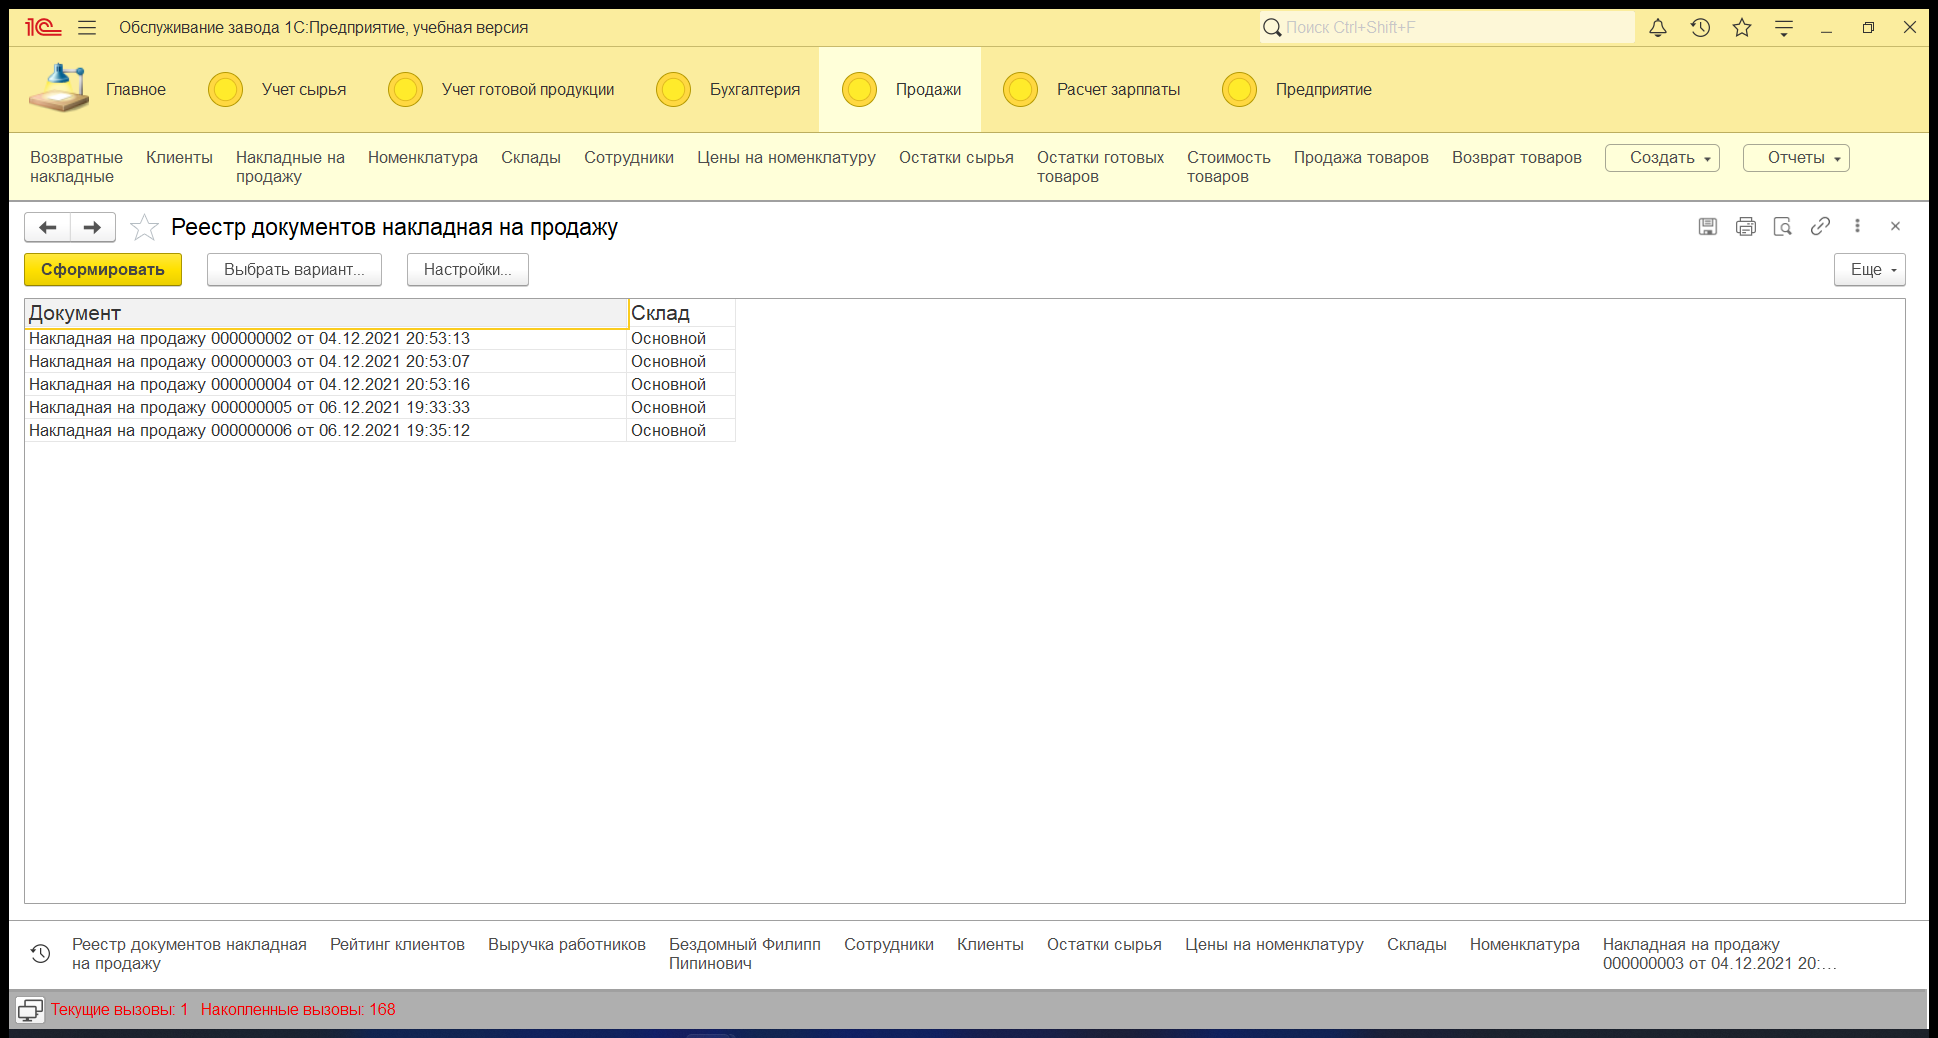
\includegraphics[scale=0.4]{Пример отчета-реестра.png}
        \caption{Пример отчета для реестра документов}
        \label{fig:registry}
    \end{figure}
    
    \item Рейтинг товаров --- отчет, в котором отображается выручка по какому-либо изготовленному товару и итоговая выручка за все реализованные <<готовые>> товары.
    
    \item Выручка работников --- отчет, в котором в виде диаграммы отражена выручка каждого работника, который реализовывал цитрусовые или изготовленную из них продукцию. Также можно посмотреть в какие дни и для какого клиента тем или иным работником была оказана услуга.
    
    \item Перечень товаров --- отчет, в котором отображается товар, группа товаров к которой он принадлежит и цена самого товара.
    
    \begin{figure}[!ht]
        \centering
        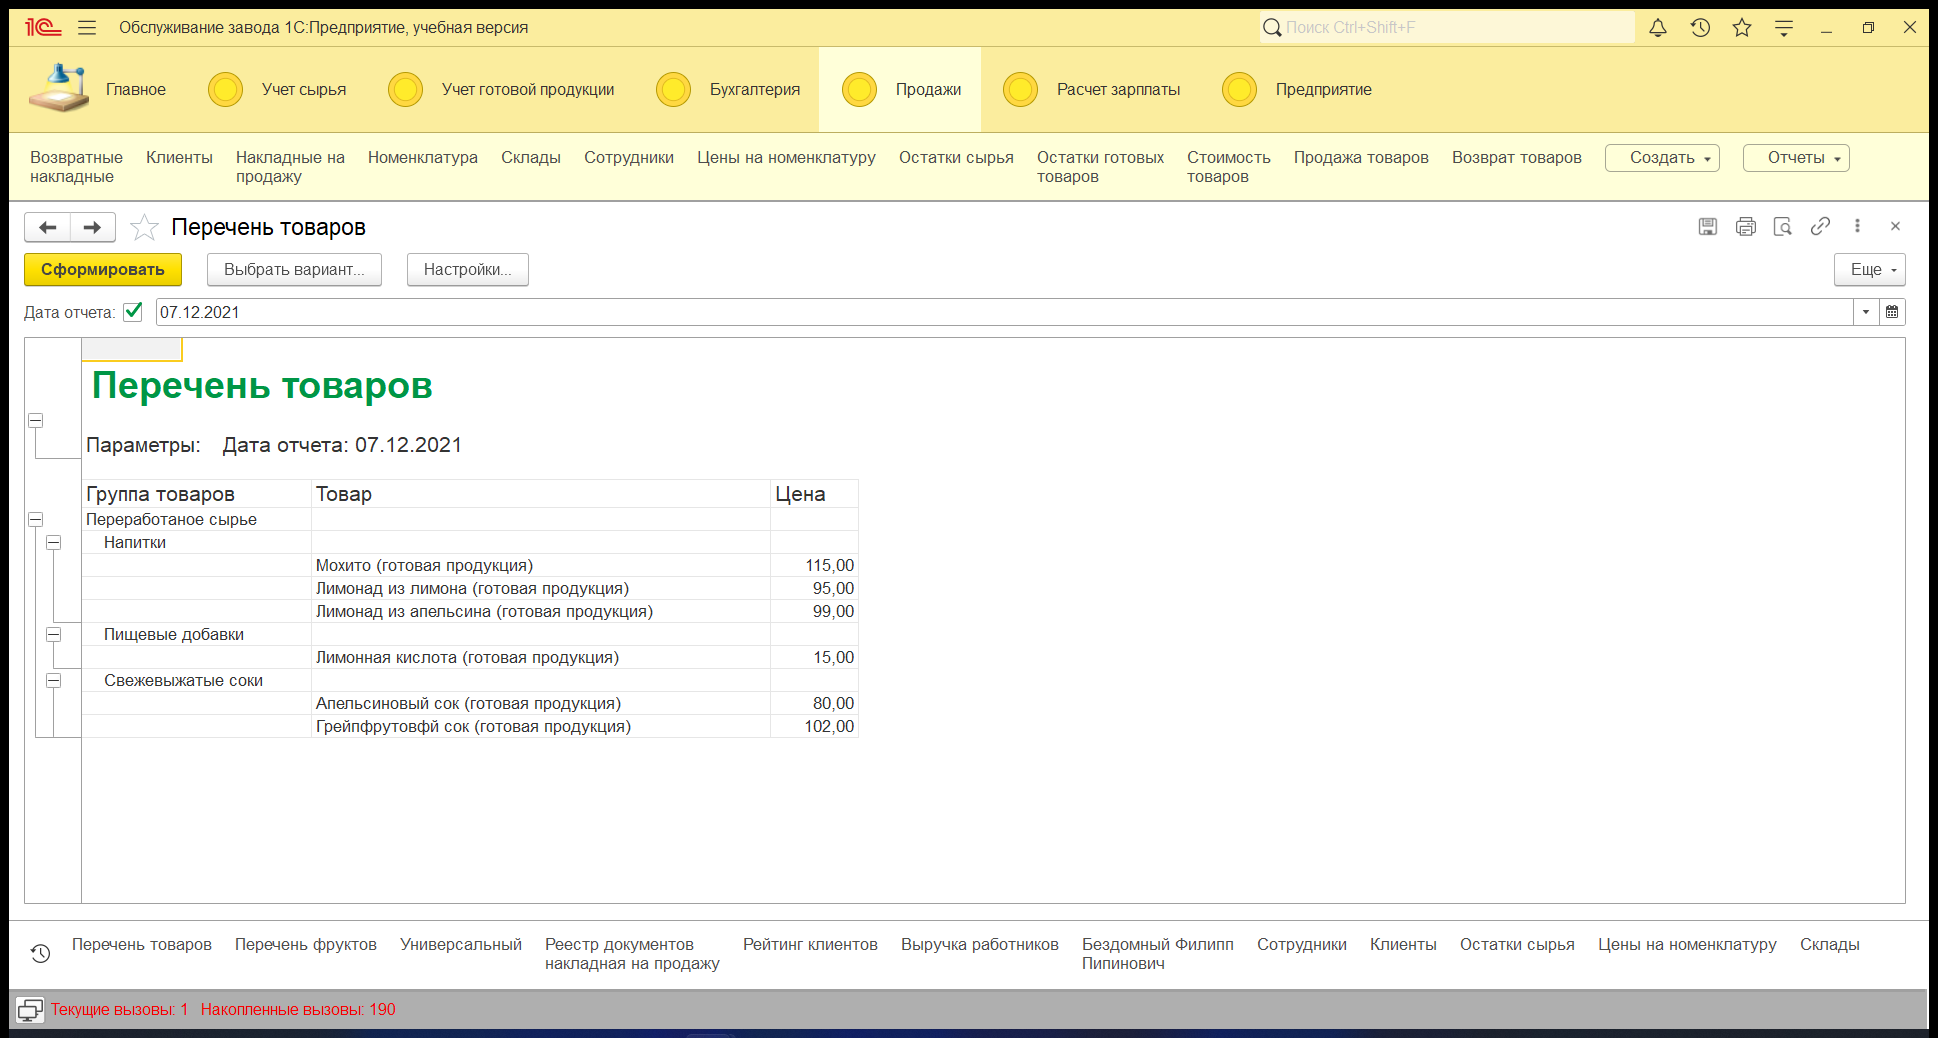
\includegraphics[scale=0.4]{Пример простого отчета.png}
        \caption{Пример простого отчета}
        \label{fig:easy_report}
    \end{figure}
    
    \item Рейтинг клиентов --- отчет, в котором посредством круговой диаграммы отображается доход от каждого из клиентов в процентном и суммарном выражении.
    
    \begin{figure}[!ht]
        \centering
        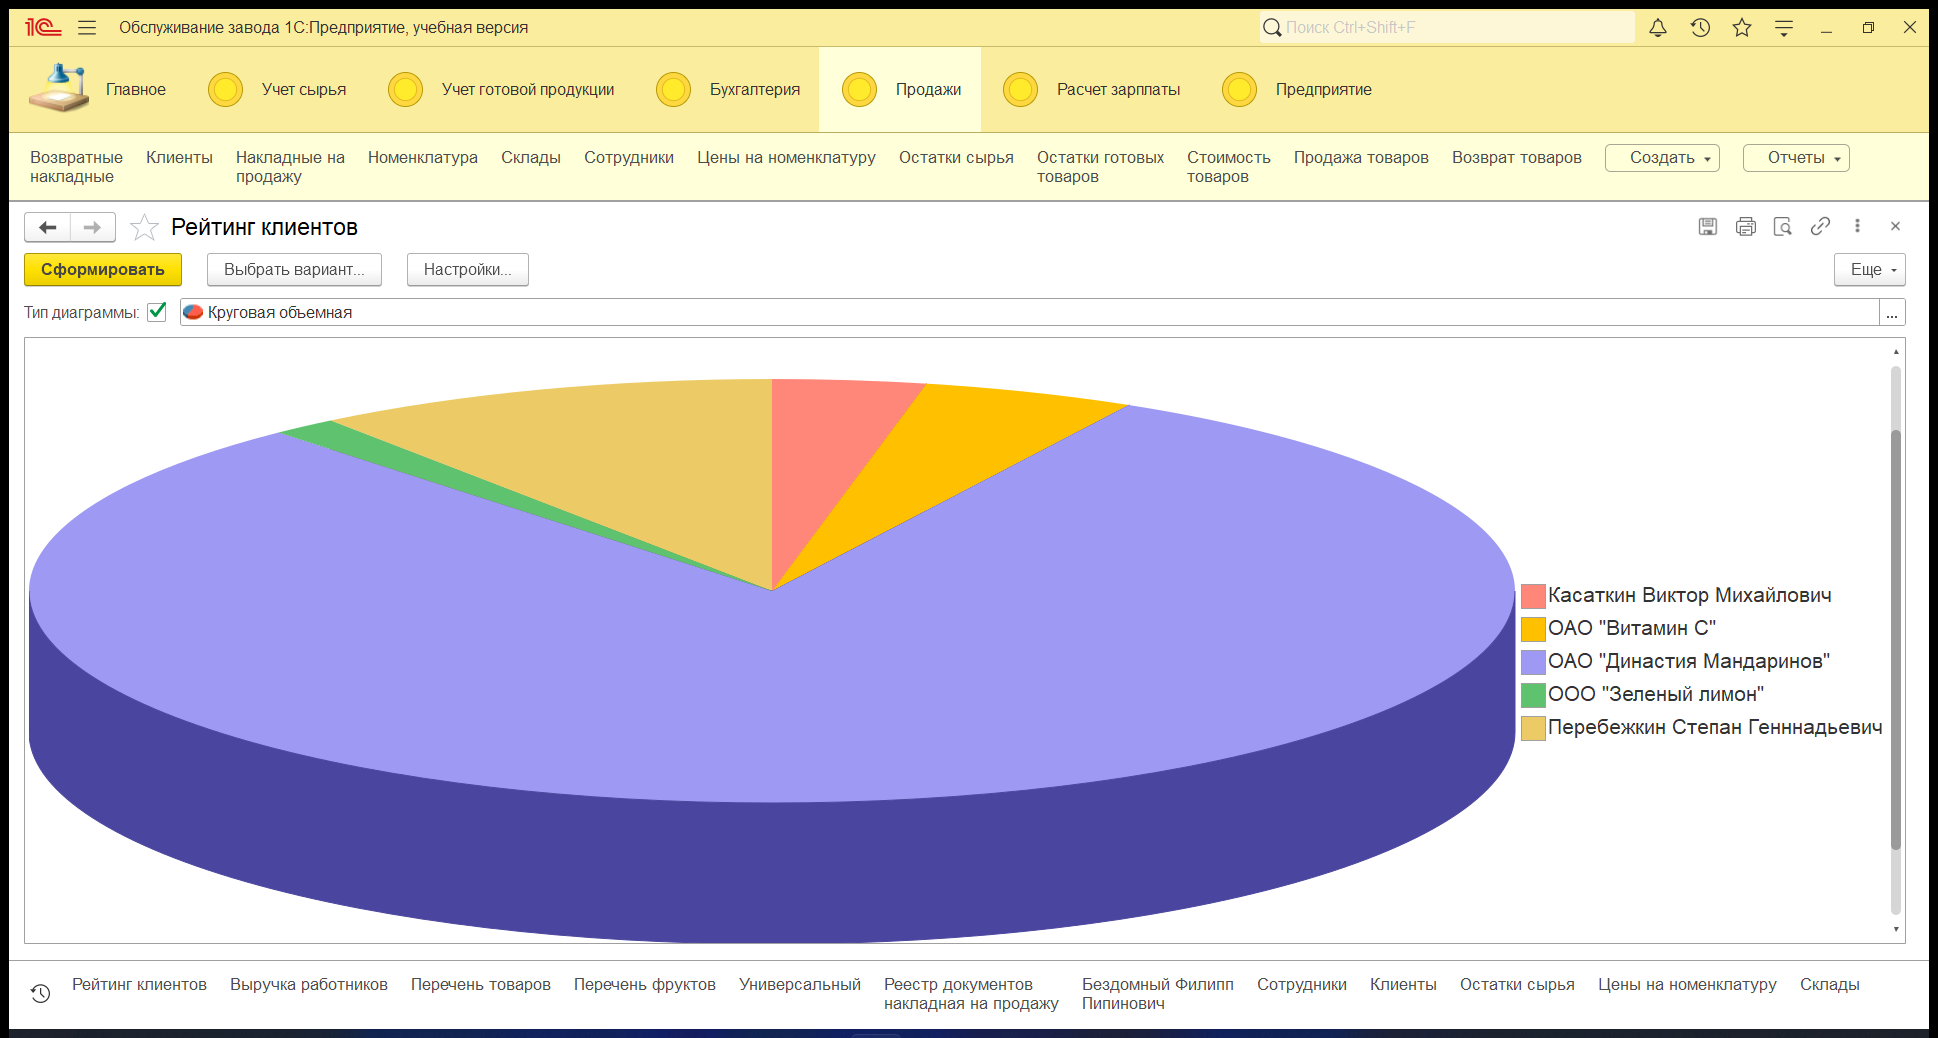
\includegraphics[scale=0.4]{Пример отчета в виде диаграммы.png}
        \caption{Пример отчета с использованием диаграммы}
        \label{fig:diagram}
    \end{figure}
    
    \item Рейтинг работников --- отчет позволяет получить полную статистику по работнику, который занимался реализацией товара (день, в который был продан тот или иной товар; количество проданных товаров; выручка от проданных товаров).
    
    \item Рейтинг фруктов --- отчет, в котором отображается выручка по определенному фрукту и итоговая выручка за все реализованные фрукты.
    
    \item Перечень фруктов --- отчет, в котором отображается фрукт, группа товаров к которой принадлежит тот или иной фрукт и цена фрукта.
    
    \item Универсальный --- отчет, в котором пользователю разрешается самому настраивать все необходимые ему для работы поля и условия отбора (рассчитано на продвинутых пользователей).
    
    \begin{figure}[!ht]
        \centering
        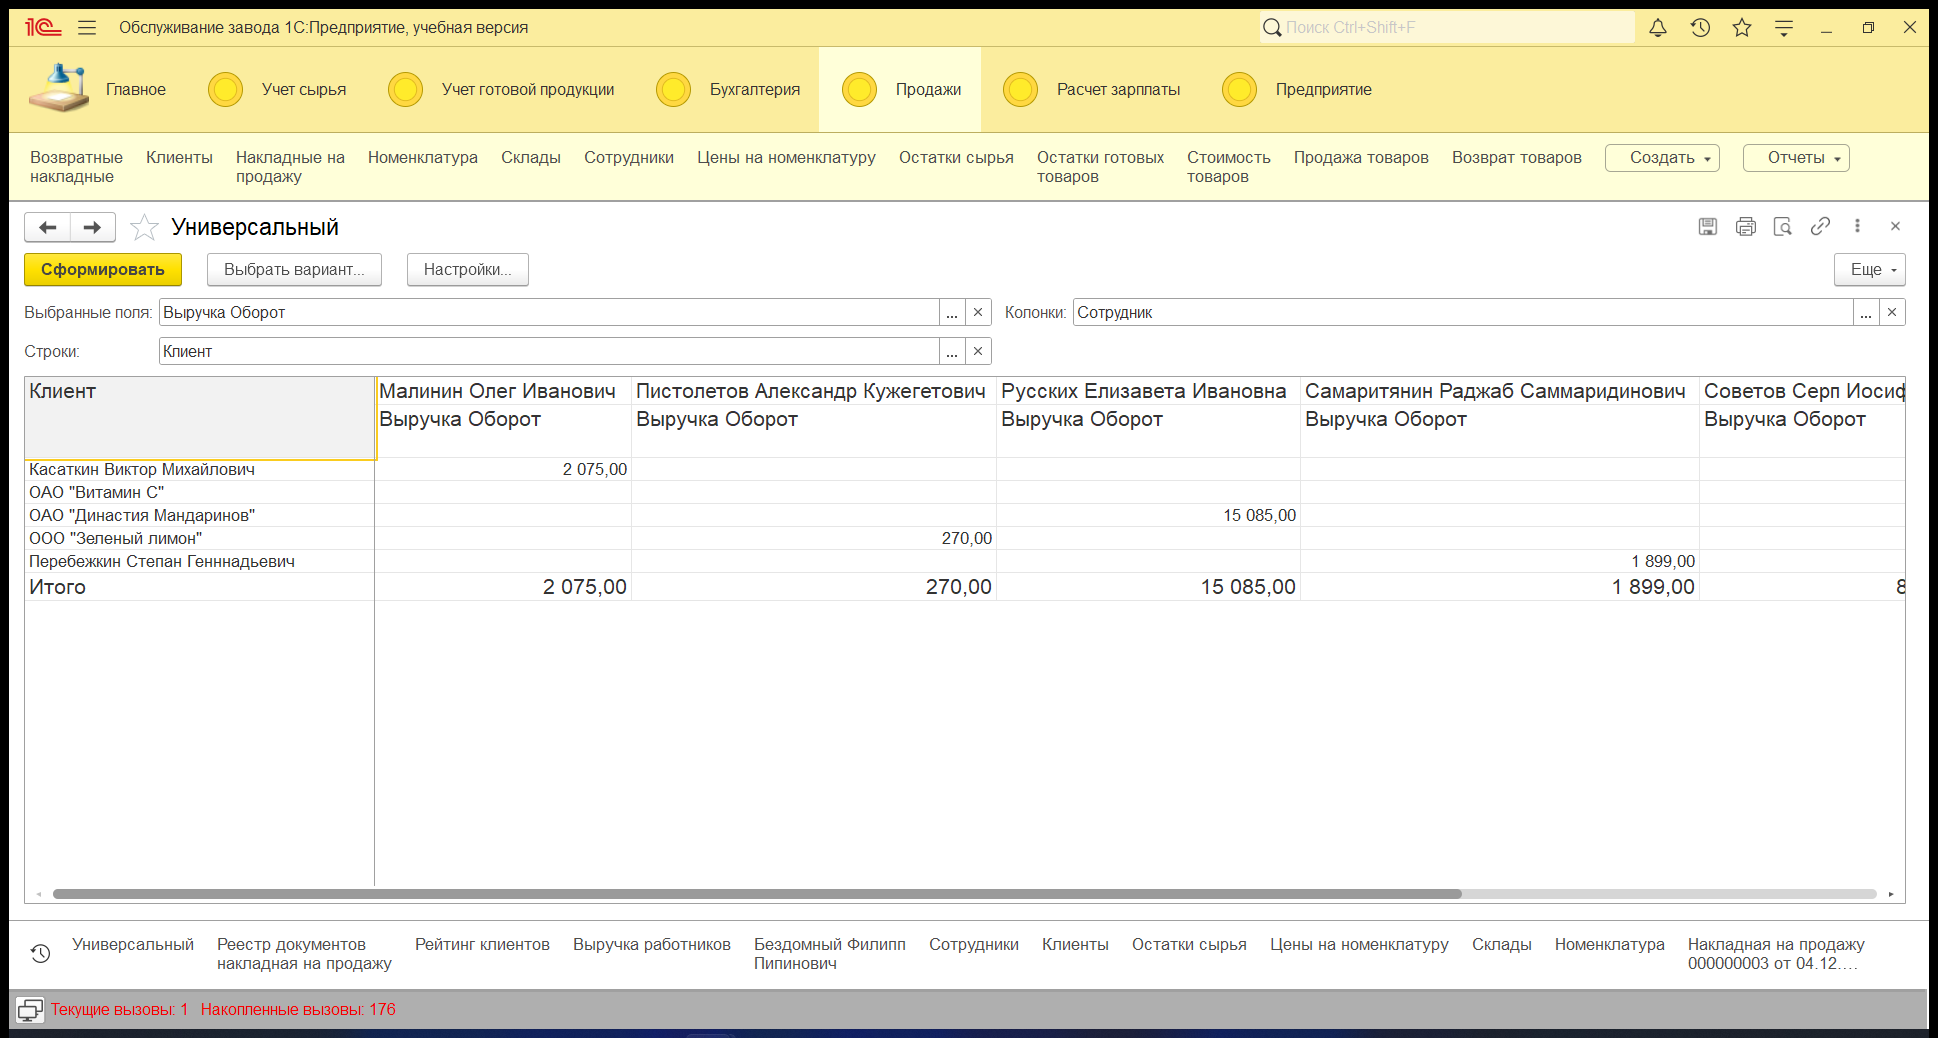
\includegraphics[scale=0.4]{Пример универсального отчета.png}
        \caption{Пример универсального отчета}
        \label{fig:universal}
    \end{figure}
\end{enumerate}

\section{Выводы}
В результате выполнения поставленной задачи была создана информационная система для завода по производству и дальнейшей переработке цитрусовых. Были реализованы все минимальные требования к информационной системе и в самой информационной системе была успешно реализована логика работы для данного предприятия.

\newpage

\newcommand{\append}[1]{
    \stepcounter{chapter}https://www.overleaf.com/project/61aeda6bdb40ec593e8d7c4f
    \begin{center}
        \chaptertitlename~\Asbuk{chapter}
    \end{center}
    \begin{center}{#1}\end{center}
    \empline
    \addcontentsline{toc}{chapter}{\Asbuk{chapter}\hspace{0.6em}~#1}}

\begin{appendices}

\section{}

\begin{verbatim}
Процедура РассчитатьСумму(СтрокаТабличнойЧасти) Экспорт
    СтрокаТабличнойЧасти.Сумма = СтрокаТабличнойЧасти.Количество *
    СтрокаТабличнойЧасти.Цена;
КонецПроцедуры
\end{verbatim}

\begin{lstlisting}[caption=Процедура РассчитатьСумму из общего модуля РаботаСДокументами]
\end{lstlisting}

\begin{verbatim}
Функция РозничнаяЦена(АктуальнаяДата, ЭлементНоменклатуры) Экспорт
    Отбор = Новый Структура( "Номенклатура" , ЭлементНоменклатуры) ;
    ЗначенияРесурсов = РегистрыСведений.Цены.ПолучитьПоследнее
    (АктуальнаяДата, Отбор) ;
    Возврат ЗначенияРесурсов.Цена;
КонецФункции
\end{verbatim}

\begin{lstlisting}[caption=Функция РозничнаяЦена из общего модуля РаботаСоСправочниками]
\end{lstlisting}

\begin{verbatim}
Процедура ОбработкаПолученияПолейПредставления(Поля, СтандартнаяОбработка)
    СтандартнаяОбработка = Ложь ;
    Поля.Добавить( "Наименование" ) ;
    Поля.Добавить( "ВидНоменклатуры" ) ;
КонецПроцедуры

Процедура ОбработкаПолученияПредставления(Данные, Представление,
    СтандартнаяОбработка)
    СтандартнаяОбработка = Ложь ;
    Если ЗначениеЗаполнено(Данные.ВидНоменклатуры) Тогда
        Представление = Данные.Наименование + " (" +
        НРег(Строка(Данные.ВидНоменклатуры) ) + ")" ;
    Иначе
        Представление = Данные.Наименование;
    КонецЕсли ;
КонецПроцедуры
\end{verbatim}

\begin{lstlisting}[caption=Процедуры в модуле менеджера справочника Номенклатура]
\end{lstlisting}

\newpage

\begin{verbatim}
Процедура ОбработкаПроведения(Отказ, Режим)
    Движения.ОстаткиСырья.Записывать = Истина; 
    Движения.СтоимостьТоваров.Записывать = Истина;
    Для Каждого ТекСтрокаФрукты Из Фрукты Цикл 
        // регистр ОстаткиСырья Приход
        Движение = Движения.ОстаткиСырья.Добавить();
        Движение.ВидДвижения = ВидДвиженияНакопления.Приход;
        Движение.Период = Дата;
        Движение.НаименованиеТовара = ТекСтрокаФрукты.НаименованиеТовара;
        Движение.Склад = Склад;
        Движение.Количество = ТекСтрокаФрукты.Количество;
        // регистр СтоимостьТоваров Приход     
        Движение = Движения.СтоимостьТоваров.Добавить();
        Движение.ВидДвижения = ВидДвиженияНакопления.Приход;
        Движение.Период = Дата;
        Движение.НаименованиеТовара = ТекСтрокаФрукты.НаименованиеТовара;
        Движение.Стоимость = ТекСтрокаФрукты.Сумма;
	КонецЦикла;
КонецПроцедуры
\end{verbatim}

\begin{lstlisting}[caption=ОбработкаПроведения из модуля объекта Приходной накладной]
\end{lstlisting}

\begin{verbatim}
Процедура ОбработкаПроведения(Отказ, Режим)
    Движения.ОстаткиГотовыхТоваров.Записывать = Истина; 
    Движения.СтоимостьТоваров.Записывать = Истина;
    Для Каждого ТекСтрокаПроизведенныеТовары Из ПроизведенныеТовары Цикл 
        // регистр ОстаткиГотовыхТоваров Приход
        Движение = Движения.ОстаткиГотовыхТоваров.Добавить();
        Движение.ВидДвижения = ВидДвиженияНакопления.Приход;
        Движение.Период = Дата;
        Движение.НаименованиеТовара =
        ТекСтрокаПроизведенныеТовары.НаименованиеТовара;
        Движение.Склад = Склад;
        Движение.Количество = ТекСтрокаПроизведенныеТовары.Количество;
        // регистр СтоимостьТоваров Приход                                   
        Движение = Движения.СтоимостьТоваров.Добавить();
        Движение.ВидДвижения = ВидДвиженияНакопления.Приход;
        Движение.Период = Дата;
        Движение.НаименованиеТовара =
        ТекСтрокаПроизведенныеТовары.НаименованиеТовара;
        Движение.Стоимость = ТекСтрокаПроизведенныеТовары.Сумма;
    КонецЦикла;
КонецПроцедуры
\end{verbatim}

\begin{lstlisting}[caption=ОбработкаПроведения из модуля объекта Товараной накладной]
\end{lstlisting}

\begin{verbatim}
Процедура ОбработкаПроведения(Отказ, Режим) 
    Движения.ОстаткиСырья.Записывать = Истина;       
    Движения.ОстаткиГотовыхТоваров.Записывать = Истина;	  
    Движения.СтоимостьТоваров.Записывать = Истина; 
    Движения.ПродажаТоваров.Записывать = Истина ;                                      
    // Создать менеджер временных таблиц
    МенеджерВТ = Новый МенеджерВременныхТаблиц;
    #Область НоменклатураДокумента
    Запрос = Новый Запрос;
    // Укажем, какой менеджер временных таблиц использует этот запрос
    Запрос.МенеджерВременныхТаблиц = МенеджерВТ;

    Запрос.Текст = 
        "ВЫБРАТЬ
        |	НакладнаяНаПродажуПроданныеТовары.
        Наименовани Товара КАК НаименованиеТовара,
        |	НакладнаяНаПродажуПроданныеТовары.НаименованиеТовара.
        ВидНоменклатуры КАК ВидНоменклатуры,
        |	СУММА(НакладнаяНаПродажуПроданныеТовары.Количество)
        КАК КоличествоВДокументе,
        |	СУММА(НакладнаяНаПродажуПроданныеТовары.Сумма)
        КАК СуммаВДокументе
        |ПОМЕСТИТЬ НоменклатураДокумента
        |ИЗ
        |	Документ.НакладнаяНаПродажу.ПроданныеТовары
        КАК НакладнаяНаПродажуПроданныеТовары
        |ГДЕ
        |	НакладнаяНаПродажуПроданныеТовары.Ссылка = &Ссылка
        |
        |СГРУППИРОВАТЬ ПО
        |	НакладнаяНаПродажуПроданныеТовары.Наименовани
        Товара,
        |	НакладнаяНаПродажуПроданныеТовары.Наименовани
        Товара.ВидНоменклатуры";
	
    Запрос.УстановитьПараметр("Ссылка", Ссылка);
	
    РезультатЗапроса = Запрос.Выполнить();
    #КонецОбласти
    #Область ДвиженияДокумента
    Запрос2 = Новый Запрос;
    Запрос2.МенеджерВременныхТаблиц = МенеджерВТ;
    Запрос2.Текст = "ВЫБРАТЬ
                    |	НоменклатураДокумента.НаименованиеТовара
                    КАК НаименованиеТовара,
                    |	НоменклатураДокумента.ВидНоменклатуры
                    КАК ВидНоменклатуры,
                    |	НоменклатураДокумента.КоличествоВДокументе
                    КАК КоличествоВДокументе,
                    |	НоменклатураДокумента.СуммаВДокументе
                    КАК СуммаВДокументе,
                    |	ЕСТЬNULL(СтоимостьТоваровОстатки.СтоимостьОстаток, 0)
                    КАК Стоимость,
                    |	ЕСТЬNULL(ОстаткиСырьяОстатки.КоличествоОстаток, 0)
                    КАК КоличествоСырья,
                    |	ЕСТЬNULL(ОстаткиГотовыхТоваровОстатки
                    КоличествоОстаток, 0) КАК КоличествоГотовыхТоваров
                    |ИЗ
                    |	НоменклатураДокумента КАК НоменклатураДокумента
                    |		ЛЕВОЕ СОЕДИНЕНИЕ РегистрНакопления.СтоимостьТоваров.
                    Остатки(
                    |				,
                    |				НаименованиеТовара В
                    |					(ВЫБРАТЬ
                    |						НоменклатураДокумента.НаименованиеТовара
                    |					ИЗ
                    |						НоменклатураДокумента)) КАК
                    СтоимостьТоваровОстатки
                    |		ПО НоменклатураДокумента.НаименованиеТовара =
                    СтоимостьТоваровОстатки.НаименованиеТовара
                    |		ЛЕВОЕ СОЕДИНЕНИЕ РегистрНакопления.ОстаткиСырья.
                    Остатки(
                    |				,
                    |				НаименованиеТовара В
                    |					(ВЫБРАТЬ
                    |						НоменклатураДокумента.НаименованиеТовара
                    |					ИЗ
                    |						НоменклатураДокумента)) КАК ОстаткиСырьяОстатки
                    |		ПО НоменклатураДокумента.НаименованиеТовара =
                    ОстаткиСырьяОстатки.НаименованиеТовара
                    |		ЛЕВОЕ СОЕДИНЕНИЕ РегистрНакопления.
                    ОстаткиГотовыхТоваров.Остатки(
                    |				,
                    |				НаименованиеТовара В
                    |					(ВЫБРАТЬ
                    |						НоменклатураДокумента.НаименованиеТовара
                    |					ИЗ
                    |						НоменклатураДокумента))
                    КАК ОстаткиГотовыхТоваровОстатки
                    |		ПО НоменклатураДокумента.НаименованиеТовара =
                    ОстаткиГотовыхТоваровОстатки.НаименованиеТовара" ;
    // Установим необходимость блокировки данных в регистрах
    СтоимостьТоваров и ОстаткиСырья и ОстаткиГотовыхТоваров
    Движения.СтоимостьТоваров.БлокироватьДляИзменения = Истина;
    Движения.ОстаткиСырья.БлокироватьДляИзменения = Истина;
    Движения.ОстаткиГотовыхТоваров.БлокироватьДляИзменения = Истина;
    // Запишем пустые наборы записей, чтобы читать остатки без учета данных
    в документе
    Движения.СтоимостьТоваров.Записать();
    Движения.ОстаткиСырья.Записать();
    Движения.ОстаткиГотовыхТоваров.Записать();
    РезультатЗапроса = Запрос2. Выполнить ( ) ;
    ВыборкаДетальныеЗаписи = РезультатЗапроса.Выбрать();
	
    Пока ВыборкаДетальныеЗаписи.Следующий() Цикл  
        Если ВыборкаДетальныеЗаписи.КоличествоСырья = 0 Тогда
            СтоимостьСырья = 0 ;
        Иначе
            СтоимостьСырья = ВыборкаДетальныеЗаписи.Стоимость /
            ВыборкаДетальныеЗаписи.КоличествоСырья;	
        КонецЕсли;
        Если ВыборкаДетальныеЗаписи.КоличествоГотовыхТоваров = 0 Тогда
            СтоимостьТовара = 0 ;
        Иначе    
            СтоимостьТовара = ВыборкаДетальныеЗаписи.Стоимость /
            ВыборкаДетальныеЗаписи.КоличествоГотовыхТоваров;
		КонецЕсли ;                                               
        Если ВыборкаДетальныеЗаписи.ВидНоменклатуры = Перечисления.
        ВидыНоменклатуры.Сырье Тогда   
            // регистр ОстаткиСырья Расход
            Движение = Движения.ОстаткиСырья.Добавить();
            Движение.ВидДвижения = ВидДвиженияНакопления.Расход;
            Движение.Период = Дата;
            Движение.НаименованиеТовара = ВыборкаДетальныеЗаписи.
            НаименованиеТовара;
            Движение.Склад = Склад;
            Движение.Количество =
            ВыборкаДетальныеЗаписи.КоличествоВДокументе; 
            // регистр СтоимостьТоваров Расход
            Движение = Движения.СтоимостьТоваров.Добавить( ) ;
            Движение.ВидДвижения = ВидДвиженияНакопления.Расход;
            Движение.Период = Дата;
            Движение.НаименованиеТовара = ВыборкаДетальныеЗаписи.
            НаименованиеТовара;
            Движение.Стоимость = ВыборкаДетальныеЗаписи.КоличествоВДокументе
            * СтоимостьСырья;
            // регистр ПродажаТоваров		
            Движение = Движения.ПродажаТоваров.Добавить( ) ;
            Движение.Период = Дата;
            Движение.НаименованиеТовара = ВыборкаДетальныеЗаписи.
            НаименованиеТовара;
            Движение.Клиент = Клиент;
            Движение.Сотрудник = Сотрудник;
            Движение.Количество =
            ВыборкаДетальныеЗаписи.КоличествоВДокументе;
            Движение.Выручка = ВыборкаДетальныеЗаписи.СуммаВДокументе;
            Движение.Стоимость = СтоимостьСырья *
            ВыборкаДетальныеЗаписи.КоличествоВДокументе;
        Иначе      
            // регистр ОстаткиГотовыхТоваров Расход  
            Движение = Движения.ОстаткиГотовыхТоваров.Добавить();
            Движение.ВидДвижения = ВидДвиженияНакопления.Расход;
            Движение.Период = Дата;
            Движение.НаименованиеТовара = ВыборкаДетальныеЗаписи.
            НаименованиеТовара;
            Движение.Склад = Склад;
            Движение.Количество =
            ВыборкаДетальныеЗаписи.КоличествоВДокументе;  
            // регистр СтоимостьТоваров Расход
            Движение = Движения.СтоимостьТоваров.Добавить( ) ;
            Движение.ВидДвижения = ВидДвиженияНакопления.Расход;
            Движение.Период = Дата;
            Движение.НаименованиеТовара = ВыборкаДетальныеЗаписи.
            НаименованиеТовара;
            Движение.Стоимость = ВыборкаДетальныеЗаписи.КоличествоВДокументе
            * СтоимостьТовара;  ;
            // регистр ПродажаТоваров		
            Движение = Движения.ПродажаТоваров.Добавить( ) ;
            Движение.Период = Дата;
            Движение.НаименованиеТовара = ВыборкаДетальныеЗаписи.
            НаименованиеТовара;
            Движение.Клиент = Клиент;
            Движение.Сотрудник = Сотрудник;
            Движение.Количество = ВыборкаДетальныеЗаписи.
            КоличествоВДокументе;
            Движение.Выручка = ВыборкаДетальныеЗаписи.СуммаВДокументе;
            Движение.Стоимость = СтоимостьТовара *
            ВыборкаДетальныеЗаписи.КоличествоВДокументе;
        КонецЕсли;
    КонецЦикла;
    Движения.Записать( ) ;
    #КонецОбласти
    #Область КонтрольОстатков
    Если Режим = РежимПроведенияДокумента.Оперативный Тогда
        // Проверить отрицательные остатки 
        Запрос3 = Новый Запрос;
        Запрос3.МенеджерВременныхТаблиц = МенеджерВТ;
        Запрос3.Текст = "ВЫБРАТЬ
                        |	ОстаткиСырьяОстатки.НаименованиеТовара
                        КАК НаименованиеТовара,
                        |	ОстаткиСырьяОстатки.КоличествоОстаток
                        КАК КоличествоОстаток
                        |ИЗ
                        |	РегистрНакопления.ОстаткиСырья.Остатки(
                        |			,
                        |			НаименованиеТовара В
                        |					(ВЫБРАТЬ
                        |						НоменклатураДокумента.НаименованиеТовара
                        |					ИЗ
                        |						НоменклатураДокумента)
                        |				И Склад = &Склад) КАК ОстаткиСырьяОстатки
                        |ГДЕ
                        |	ОстаткиСырьяОстатки.КоличествоОстаток < 0" ;
        Запрос3.УстановитьПараметр( "Склад" , Склад) ;
        РезультатЗапроса = Запрос3. Выполнить ( ) ;
        ВыборкаДетальныеЗаписи = РезультатЗапроса.Выбрать( ) ;
        Пока ВыборкаДетальныеЗаписи.Следующий( ) Цикл
            Сообщение = Новый СообщениеПользователю( ) ;
            Сообщение.Текст = "Не хватает " + Строка( -
            ВыборкаДетальныеЗаписи.КоличествоОстаток) +
            " единиц материала " "" +
            ВыборкаДетальныеЗаписи.НаименованиеТовара + "" "" ;
            Сообщение.Сообщить( ) ;
            Отказ = Истина ;
        КонецЦикла ;
        Запрос4 = Новый Запрос;
        Запрос4.МенеджерВременныхТаблиц = МенеджерВТ;
        Запрос4.Текст = "ВЫБРАТЬ
                        |	ОстаткиГотовыхТоваровОстатки.НаименованиеТовара
                        КАК НаименованиеТовара,
                        |	ОстаткиГотовыхТоваровОстатки.КоличествоОстаток
                        КАК КоличествоОстаток
                        |ИЗ
                        |	РегистрНакопления.ОстаткиГотовыхТоваров.Остатки(
                        |			,
                        |			НаименованиеТовара В
                        |					(ВЫБРАТЬ
                        |						НоменклатураДокумента.НаименованиеТовара
                        |					ИЗ
                        |						НоменклатураДокумента)
                        |				И Склад = &Склад) КАК ОстаткиГотовыхТоваровОстатки
                        |ГДЕ
                        |	ОстаткиГотовыхТоваровОстатки.КоличествоОстаток
                        < 0" ;
        Запрос4.УстановитьПараметр( "Склад" , Склад) ;
        РезультатЗапроса = Запрос4. Выполнить ( ) ;
        ВыборкаДетальныеЗаписи = РезультатЗапроса.Выбрать( ) ;
        Пока ВыборкаДетальныеЗаписи.Следующий( ) Цикл
            Сообщение = Новый СообщениеПользователю( ) ;
            Сообщение.Текст = "Не хватает " + Строка( -
            ВыборкаДетальныеЗаписи.КоличествоОстаток) +
            " единиц материала " "" +
            ВыборкаДетальныеЗаписи.НаименованиеТовара + "" "" ;
            Сообщение.Сообщить( ) ;
            Отказ = Истина ;
        КонецЦикла ;
    КонецЕсли ; 
    #КонецОбласти
КонецПроцедуры
\end{verbatim}

\begin{lstlisting}[caption=ОбработкаПроведения из модуля  объекта Накладной на продажу]
\end{lstlisting}

\begin{verbatim}
Процедура ОбработкаПроведения(Отказ, Режим)
    Движения.ВозвратТоваров.Записывать = Истина; 
    Движения.СтоимостьТоваров.Записывать = Истина;
    Для Каждого ТекСтрокаПроданныеТовары Из ПроданныеТовары Цикл
        // регистр ВозвратТоваров Приход
        Движение = Движения.ВозвратТоваров.Добавить();
        Движение.ВидДвижения = ВидДвиженияНакопления.Приход;
        Движение.Период = Дата;
        Движение.НаименованиеТовара =
        ТекСтрокаПроданныеТовары.НаименованиеТовара;
        Движение.Склад = Склад;
        Движение.Количество = ТекСтрокаПроданныеТовары.Количество;     
        // регистр СтоимостьТоваров Приход     
        Движение = Движения.СтоимостьТоваров.Добавить();
        Движение.ВидДвижения = ВидДвиженияНакопления.Приход;
        Движение.Период = Дата;
        Движение.НаименованиеТовара =
        ТекСтрокаПроданныеТовары.НаименованиеТовара;
        Движение.Стоимость = ТекСтрокаПроданныеТовары.Сумма;
    КонецЦикла;
КонецПроцедуры
\end{verbatim}

\begin{lstlisting}[caption=ОбработкаПроведения из модуля объекта Возвратной накладной]
\end{lstlisting}

\begin{verbatim}
Процедура ОбработкаПроведения(Отказ, Режим)
    Движения.СписаниеТоваров.Записывать = Истина;    
    Движения.СтоимостьТоваров.Записывать = Истина;
    Для Каждого ТекСтрокаТовары Из Товары Цикл
        // регистр СписаниеТоваров Расход
        Движение = Движения.СписаниеТоваров.Добавить();
        Движение.ВидДвижения = ВидДвиженияНакопления.Расход;
        Движение.Период = Дата;
        Движение.НаименованиеТовара = ТекСтрокаТовары.НаименованиеТовара;
        Движение.Склад = Склад;
        Движение.Количество = ТекСтрокаТовары.Количество;
        // регистр СтоимостьТоваров Приход     
        Движение = Движения.СтоимостьТоваров.Добавить();
        Движение.ВидДвижения = ВидДвиженияНакопления.Приход;
        Движение.Период = Дата;
        Движение.НаименованиеТовара = ТекСтрокаТовары.НаименованиеТовара;
        Движение.Стоимость = ТекСтрокаТовары.Сумма;
    КонецЦикла;
КонецПроцедуры
\end{verbatim}

\begin{lstlisting}[caption=ОбработкаПроведения из Накладной по истечению срока хранения]
\end{lstlisting}

\begin{verbatim}
&НаКлиенте
Процедура ФруктыКоличествоПриИзменении(Элемент)
    СтрокаТабличнойЧасти = Элементы.Фрукты.ТекущиеДанные;
    РаботаСДокументами.РассчитатьСумму(СтрокаТабличнойЧасти) ;
КонецПроцедуры

&НаКлиенте
Процедура ФруктыЦенаПриИзменении(Элемент)
    СтрокаТабличнойЧасти = Элементы.Фрукты.ТекущиеДанные;
    РаботаСДокументами.РассчитатьСумму(СтрокаТабличнойЧасти) ;
КонецПроцедуры
\end{verbatim}

\begin{lstlisting}[caption=Процедуры для автоматического пересчета суммы (Приходная накладная)]
\end{lstlisting}

\begin{verbatim}
&НаКлиенте
Процедура ПроизведенныеТоварыКоличествоПриИзменении(Элемент)
    СтрокаТабличнойЧасти = Элементы.ПроизведенныеТовары.ТекущиеДанные;
    РаботаСДокументами.РассчитатьСумму(СтрокаТабличнойЧасти) ;
КонецПроцедуры

&НаКлиенте
Процедура ПроизведенныеТоварыЦенаПриИзменении(Элемент)
    СтрокаТабличнойЧасти = Элементы.ПроизведенныеТовары.ТекущиеДанные;
    РаботаСДокументами.РассчитатьСумму(СтрокаТабличнойЧасти) ;
КонецПроцедуры
\end{verbatim}

\begin{lstlisting}[caption=Процедуры для автоматического пересчета суммы (Товарная накладная)]
\end{lstlisting}

\begin{verbatim}
&НаКлиенте
Процедура ПроданныеТоварыНаименованиеТовараПриИзменении(Элемент) 
    СтрокаТабличнойЧасти = Элементы.ПроданныеТовары.ТекущиеДанные;
    СтрокаТабличнойЧасти.Цена =
    РаботаСоСправочниками.РозничнаяЦена(Объект.Дата,
    СтрокаТабличнойЧасти.НаименованиеТовара) ;
    РаботаСДокументами.РассчитатьСумму(СтрокаТабличнойЧасти) ;
КонецПроцедуры

&НаКлиенте
Процедура ПроданныеТоварыКоличествоПриИзменении(Элемент)
    СтрокаТабличнойЧасти = Элементы.ПроданныеТовары.ТекущиеДанные;
    РаботаСДокументами.РассчитатьСумму(СтрокаТабличнойЧасти) ;
КонецПроцедуры

&НаКлиенте
Процедура ПроданныеТоварыЦенаПриИзменении(Элемент)
    СтрокаТабличнойЧасти = Элементы.ПроданныеТовары.ТекущиеДанные;
    РаботаСДокументами.РассчитатьСумму(СтрокаТабличнойЧасти) ;
КонецПроцедуры
\end{verbatim}

\begin{lstlisting}[caption=Пересчет суммы и подстановка цен на товары (Накладная на продажу)]
\end{lstlisting}

\begin{verbatim}
&НаКлиенте
Процедура ПроданныеТоварыНаименованиеТовараПриИзменении(Элемент)
    СтрокаТабличнойЧасти = Элементы.ПроданныеТовары.ТекущиеДанные;
    СтрокаТабличнойЧасти.Цена =
    РаботаСоСправочниками.РозничнаяЦена(Объект.Дата,
    СтрокаТабличнойЧасти.НаименованиеТовара) ;
    РаботаСДокументами.РассчитатьСумму(СтрокаТабличнойЧасти) ;
КонецПроцедуры

&НаКлиенте
Процедура ПроданныеТоварыКоличествоПриИзменении(Элемент)
    СтрокаТабличнойЧасти = Элементы.ПроданныеТовары.ТекущиеДанные;
    РаботаСДокументами.РассчитатьСумму(СтрокаТабличнойЧасти) ;
КонецПроцедуры

&НаКлиенте
Процедура ПроданныеТоварыЦенаПриИзменении(Элемент)
    СтрокаТабличнойЧасти = Элементы.ПроданныеТовары.ТекущиеДанные;
    РаботаСДокументами.РассчитатьСумму(СтрокаТабличнойЧасти) ;
КонецПроцедуры
\end{verbatim}

\begin{lstlisting}[caption=Пересчет суммы и подстановка цен на товары (Возвратная накладная)]
\end{lstlisting}

\begin{verbatim}
&НаКлиенте
Процедура ТоварыНаименованиеТовараПриИзменении(Элемент)
    СтрокаТабличнойЧасти = Элементы.Товары.ТекущиеДанные;
    СтрокаТабличнойЧасти.Цена =
    РаботаСоСправочниками.РозничнаяЦена(Объект.Дата,
    СтрокаТабличнойЧасти.НаименованиеТовара) ;
    РаботаСДокументами.РассчитатьСумму(СтрокаТабличнойЧасти) ;
КонецПроцедуры

&НаКлиенте
Процедура ТоварыКоличествоПриИзменении(Элемент)
    СтрокаТабличнойЧасти = Элементы.Товары.ТекущиеДанные;
    РаботаСДокументами.РассчитатьСумму(СтрокаТабличнойЧасти) ;
КонецПроцедуры

&НаКлиенте
Процедура ТоварыЦенаПриИзменении(Элемент)
    СтрокаТабличнойЧасти = Элементы.Товары.ТекущиеДанные;
    РаботаСДокументами.РассчитатьСумму(СтрокаТабличнойЧасти) ;
КонецПроцедуры
\end{verbatim}

\begin{lstlisting}[caption=Модуль формы документа Накладная по истечению срока хранения]
\end{lstlisting}

\begin{verbatim}
ВЫБРАТЬ
    ОстаткиСырьяОстаткиИОбороты.НаименованиеТовара КАК НаименованиеТовара,
    ОстаткиСырьяОстаткиИОбороты.Склад КАК Склад,
    ОстаткиСырьяОстаткиИОбороты.КоличествоНачальныйОстаток
    КАК НачальныйОстаток,
    ОстаткиСырьяОстаткиИОбороты.КоличествоПриход КАК Приход,
    ОстаткиСырьяОстаткиИОбороты.КоличествоРасход КАК Расход,
    ОстаткиСырьяОстаткиИОбороты.КоличествоКонечныйОстаток
    КАК КонечныйОстаток
ИЗ
    РегистрНакопления.ОстаткиСырья.ОстаткиИОбороты
    КАК ОстаткиСырьяОстаткиИОбороты
\end{verbatim}

\begin{lstlisting}[caption=Запрос к отчету <<Сырье>>]
\end{lstlisting}

\begin{verbatim}
ВЫБРАТЬ
    ОстаткиГотовыхТоваровОстаткиИОбороты.НаименованиеТовара
    КАК НаименованиеТовара,
    ОстаткиГотовыхТоваровОстаткиИОбороты.Склад КАК Склад,
    ОстаткиГотовыхТоваровОстаткиИОбороты.КоличествоНачальныйОстаток
    КАК НачальныйОстаток,
    ОстаткиГотовыхТоваровОстаткиИОбороты.КоличествоПриход КАК Приход,
    ОстаткиГотовыхТоваровОстаткиИОбороты.КоличествоРасход КАК Расход,
    ОстаткиГотовыхТоваровОстаткиИОбороты.КоличествоКонечныйОстаток
    КАК КонечныйОстаток
ИЗ
    РегистрНакопления.ОстаткиГотовыхТоваров.ОстаткиИОбороты
    КАК ОстаткиГотовыхТоваровОстаткиИОбороты
\end{verbatim}

\begin{lstlisting}[caption=Запрос к отчету <<ГотоваяПродукция>>]
\end{lstlisting}

\begin{verbatim}
ВЫБРАТЬ
    НакладнаяНаПродажу.Склад КАК Склад,
    НакладнаяНаПродажу.Ссылка КАК Документ
ИЗ
    Документ.НакладнаяНаПродажу КАК НакладнаяНаПродажу

УПОРЯДОЧИТЬ ПО
    Документ
\end{verbatim}

\begin{lstlisting}[caption=Запрос к отчету <<Реестр документов Накладная на продажу>>]
\end{lstlisting}

\begin{verbatim}
ВЫБРАТЬ
    СпрНоменклатура.Ссылка КАК Товар,
    ПродажаТоваровОбороты.ВыручкаОборот КАК Выручка
ИЗ
    Справочник.Номенклатура КАК СпрНоменклатура
        ЛЕВОЕ СОЕДИНЕНИЕ РегистрНакопления.ПродажаТоваров.Обороты
        КАК ПродажаТоваровОбороты
        ПО ПродажаТоваровОбороты.НаименованиеТовара = СпрНоменклатура.Ссылка
ГДЕ
    СпрНоменклатура.ЭтоГруппа = ЛОЖЬ
    И СпрНоменклатура.ВидНоменклатуры = &ВидНоменклатуры

УПОРЯДОЧИТЬ ПО
    Выручка УБЫВ
\end{verbatim}

\begin{lstlisting}[caption=Запрос к отчету <<Рейтинг товаров>>]
\end{lstlisting}

\begin{verbatim}
ВЫБРАТЬ
    ПродажаТоваровОбороты.Сотрудник КАК Сотрудник,
    ПродажаТоваровОбороты.Период КАК Период,
    ПродажаТоваровОбороты.Клиент КАК Клиент,
    ПродажаТоваровОбороты.ВыручкаОборот КАК Выручка
ИЗ
    РегистрНакопления.ПродажаТоваров.Обороты(, , День, )
	КАК ПродажаТоваровОбороты
\end{verbatim}

\begin{lstlisting}[caption=Запрос к отчету <<Выручка работников>>]
\end{lstlisting}

\begin{verbatim}
ВЫБРАТЬ
    СпрНоменклатура.Родитель КАК ГруппаТоваров,
    СпрНоменклатура.Ссылка КАК Товар,
    ЦеныСрезПоследних.Цена КАК Цена
ИЗ
    Справочник.Номенклатура КАК СпрНоменклатура
        ЛЕВОЕ СОЕДИНЕНИЕ РегистрСведений.Цены.СрезПоследних(&ДатаОтчета, )
        КАК ЦеныСрезПоследних
        ПО ЦеныСрезПоследних.Номенклатура = СпрНоменклатура.Ссылка
ГДЕ
    СпрНоменклатура.ВидНоменклатуры = &ВидНоменклатуры
\end{verbatim}

\begin{lstlisting}[caption=Запрос к отчету <<Перечень товаров>>]
\end{lstlisting}

\begin{verbatim}
ВЫБРАТЬ
    ПродажаТоваровОбороты.Клиент КАК Клиент,
    ПродажаТоваровОбороты.ВыручкаОборот КАК Выручка,
    ПродажаТоваровОбороты.СтоимостьОборот КАК Стоимость
ИЗ
    РегистрНакопления.ПродажаТоваров.Обороты
    КАК ПродажаТоваровОбороты
\end{verbatim}

\begin{lstlisting}[caption=Запрос к отчету <<Рейтинг клиентов>>]
\end{lstlisting}

\begin{verbatim}
ВЫБРАТЬ
    ПродажаТоваровОбороты.НаименованиеТовара КАК НаименованиеТовара,
    ПродажаТоваровОбороты.Клиент КАК Клиент,
    ПродажаТоваровОбороты.Сотрудник КАК Сотрудник,
    ПродажаТоваровОбороты.КоличествоОборот КАК КоличествоОборот,
    ПродажаТоваровОбороты.ВыручкаОборот КАК ВыручкаОборот,
    ПродажаТоваровОбороты.СтоимостьОборот КАК СтоимостьОборот
ИЗ
    РегистрНакопления.ПродажаТоваров.Обороты КАК ПродажаТоваровОбороты
\end{verbatim}

\begin{lstlisting}[caption=Запрос к отчету <<Универсальный>>]
\end{lstlisting}

\begin{verbatim}
ВЫБРАТЬ
    ПродажаТоваровОбороты.Сотрудник КАК Сотрудник,
    ПродажаТоваровОбороты.КоличествоОборот КАК Количество,
    ПродажаТоваровОбороты.ВыручкаОборот КАК Выручка,
    ПродажаТоваровОбороты.Период КАК Период
ИЗ
    РегистрНакопления.ПродажаТоваров.Обороты(, , День, )
    КАК ПродажаТоваровОбороты
\end{verbatim}

\begin{lstlisting}[caption=Запрос к отчету <<Рейтинг работников>>]
\end{lstlisting}

\begin{verbatim}
ВЫБРАТЬ
    СпрНоменклатура.Ссылка КАК Фрукт,
    ПродажаТоваровОбороты.ВыручкаОборот КАК Выручка
ИЗ
    Справочник.Номенклатура КАК СпрНоменклатура
        ЛЕВОЕ СОЕДИНЕНИЕ РегистрНакопления.ПродажаТоваров.Обороты
        КАК ПродажаТоваровОбороты
        ПО (ПродажаТоваровОбороты.НаименованиеТовара =
        СпрНоменклатура.Ссылка)
ГДЕ
    СпрНоменклатура.ЭтоГруппа = ЛОЖЬ
    И СпрНоменклатура.ВидНоменклатуры = &ВидНоменклатуры

УПОРЯДОЧИТЬ ПО
    Выручка УБЫВ
\end{verbatim}

\begin{lstlisting}[caption=Запрос к отчету <<Рейтинг фруктов>>]
\end{lstlisting}

\begin{verbatim}
ВЫБРАТЬ
    СпрНоменклатура.Родитель КАК ГруппаТоваров,
    СпрНоменклатура.Ссылка КАК Фрукт,
    ЦеныСрезПоследних.Цена КАК Цена
ИЗ
    Справочник.Номенклатура КАК СпрНоменклатура
        ЛЕВОЕ СОЕДИНЕНИЕ РегистрСведений.Цены.СрезПоследних(&ДатаОтчета, )
        КАК ЦеныСрезПоследних
        ПО (ЦеныСрезПоследних.Номенклатура = СпрНоменклатура.Ссылка)
ГДЕ
    СпрНоменклатура.ВидНоменклатуры = &ВидНоменклатуры
\end{verbatim}

\begin{lstlisting}[caption=Запрос к отчету <<Перечень фруктов>>]
\end{lstlisting}
\end{appendices}

\end{document}
